\chapter{Potential Flow}

%
%  SECTION 4.1 - THE COMPLEX POTENTIAL
%

\section{The Complex Potential}

In the previous chapter, we saw that an irrotational fluid can be described by the \emph{velocity potential} $\varphi$, defined by
\begin{equation}
\vec{u} = \grad \varphi.
\end{equation}
If, instead, the fluid is both two dimensional and incompressible, it can be described by the stream function, $\psi$, defined via
\begin{equation}
\vec{u} = \grad \times (\psi \, \unit{z}).
\end{equation}
Now, if we have a two dimensional fluid that is both irrotational \emph{and} incompressible, then we can use either $\varphi$ \emph{or} $\psi$ to describe it; in Cartesian coordinates, we have
\begin{equation}
\label{eq_u_phi_psi}
u = \dfdx{\varphi}{x} = \dfdx{\psi}{y} \quad \text{and} \quad v = \dfdx{\varphi}{y} = - \dfdx{\psi}{x}.
\end{equation}

For reasons we'll learn as we go, it's very convenient to define a \emph{third} function, the \emph{complex potential} $w(z)$:
\begin{equation}
\label{eq_complex_pot}
\boxed{
w(z) = \varphi + i \psi.
}
\end{equation}
Unlike the velocity potential and the stream function, the complex potential is a function of a \emph{single} variable -- the complex number $z$.   That makes now a good time to review our knowledge of the complex plane. 

% SECTION 4.1.1 - THE COMPLEX PLANE

\subsection{The Complex Plane}

Consider a complex number $z$:
\begin{equation}
z = x + iy.
\end{equation}
We call $x$ the \emph{real part} of the complex number and $y$ the \emph{imaginary part}.  This can be represented on a Cartesian coordinate system as shown in Figure \ref{fig_complex_plane}; the $x$ axis is the real axis and the $y$ axis the imaginary.  This is called the \emph{complex plane}. 

\begin{figure}
\centering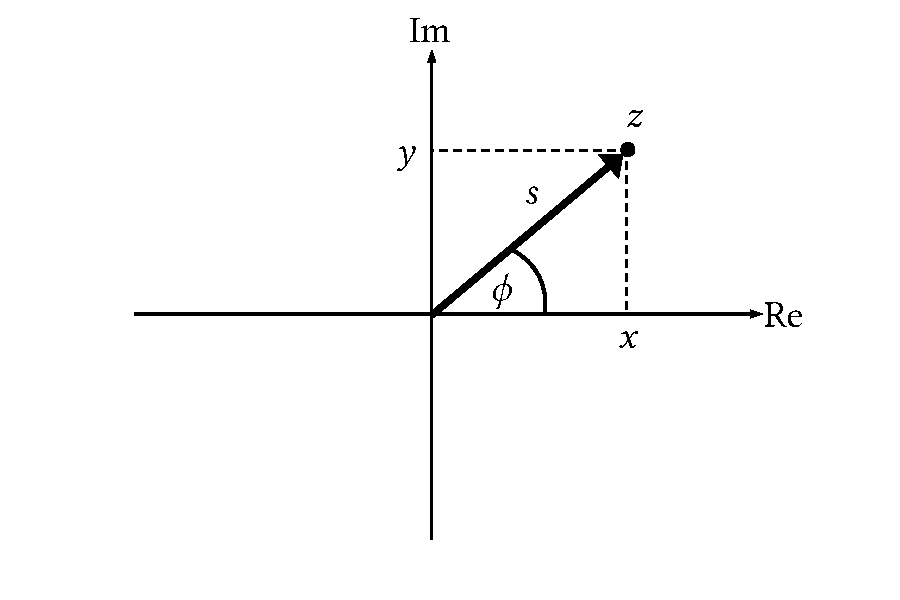
\includegraphics[width=0.7\linewidth]{Figures/Chapter4/fig_complex_plane}
\caption{The complex plane showing the complex number $z = x + iy = s \, e^{i\phi}$.}
\label{fig_complex_plane}
\end{figure}

In addition to using Cartesian coordinates, we can also write the complex number $z$ in polar coordinates; it should be clear from the figure that
\[
z = x + iy = s \cos \phi + is \sin \phi.
\]
Using Euler's famous formula,
\[
e^{i \phi} = \cos \phi + i \sin \phi,
\]
this becomes
\begin{equation}
z = s \, e^{i \phi}.
\end{equation}

Some operations, like multiplying complex numbers, are easier in polar coordinates.  Other operations are unique to complex numbers, such as taking the \emph{complex conjugate} of $z$; this means that every imaginary number $i$ becomes the negative $-i$.  The complex conjugate is denoted with a star:
\[
z^* = x - iy = s \, e^{-i\phi}.
\] 
Although we can square a complex number as normal,
\begin{equation}
\label{eq_z_squared}
z^2 = (x + iy)^2 = x^2 - y^2 + 2ixy,
\end{equation}
an operation that often comes up is the ``complex square,''
\begin{equation}
|z|^2 \equiv z^* z = (x-iy)(x+iy) = x^2 + y^2.
\end{equation}
Notice that the complex square will always give a real number.

Sometimes you'll have a complex number in the denominator of a fraction, which makes it difficult to separate the real and imaginary parts of the complex number -- something we'll do pretty frequently.  You can always get rid of the imaginary part in the denominator by multiplying by the complex conjugate:
\[
\frac{1}{x + iy} = \frac{1}{x+iy} \frac{x - iy}{x-iy} = \frac{x - iy}{x^2 + y^2}.
\]

So far, this is all pretty basic stuff, but we need at least one thing from the more advanced theory of complex analysis -- we'll be working with \emph{complex functions} $f(z)$.  Like complex numbers, complex functions can be separated into real and imaginary parts,
\[
f(z) = f(x + iy) = A(x, y) + i B(x, y),
\]
where $A(x, y)$ and $B(x, y)$ are real-valued functions.  Now, a complex function is \emph{analytic} if $A$ and $B$ are differentiable and satisfy the so-called \emph{Cauchy-Riemann conditions,}
\begin{equation}
\label{eq_cauchy_riemann}
\dfdx{A}{x} = \dfdx{B}{y} \quad \text{and} \quad \dfdx{A}{y} = - \dfdx{B}{x}.
\end{equation}
This means that the complex derivative exists, and can be written as\footnote{This is obviously a drastically shortened and simplified look at complex analysis; for more, see e.g., \emph{Mathematical Method for Physicists}, 4th edition, by Arfken and Weber, Chapter 6.}
\begin{equation}
\frac{df}{dz} = \dfdx{A}{x} + i \dfdx{B}{x} = \dfdx{B}{y} - i \dfdx{A}{y}.
\end{equation}

You might have noticed that the Cauchy-Riemann conditions look a lot like equation (\ref{eq_u_phi_psi}) -- the relationship between the velocity potential and the stream function.  This is the connection to fluid dynamics:  by construction, the complex potential $w(z)$ is an analytic complex function, which means we can write the derivative of it as
\begin{equation}
\label{eq_w_deriv}
\boxed{
\frac{dw}{dz} = \dfdx{\varphi}{x} + i \dfdx{\psi}{x} = u - iv.
}
\end{equation}
Thus the derivative of the complex potential is related to the speed of the fluid by
\[
|\vec{u} | = \left| \frac{dw}{dz} \right| = \sqrt{ \left( \frac{dw}{dz} \right)^* \left( \frac{dw}{dz} \right) }.
\]
This gives us a powerful tool to examine some pretty complicated flows.


% SECTION 4.1.2- BASIC FLOWS

\subsection{Basic Flows}

Although we're restricted to two dimensional, incompressible, irrotational flows, the complex potential is nonetheless a useful description of fluid flow in a variety of cases.  We'll start here with four basic flows, and will build up to fluid flow around a wing of an airplane, all the while using tools of complex analysis.

\begin{figure}
\centering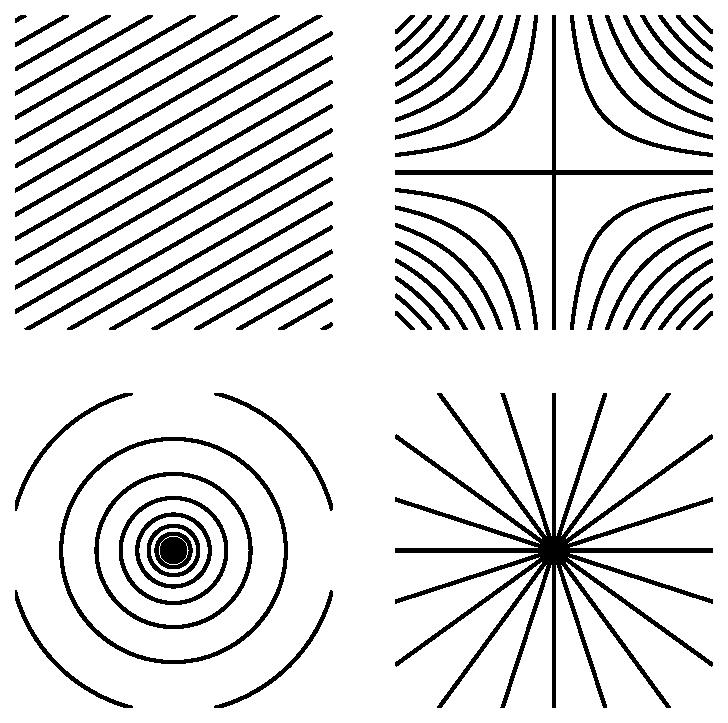
\includegraphics[width=0.6\linewidth]{Figures/Chapter4/fig_basic_flows}
\caption{Four basic potential flows.  Upper left: uniform flow at an angle $\alpha$.  Upper right: flow about a stagnation point.  Lower left: a line vortex.  Lower right: a line source.}
\label{fig_basic_flows}
\end{figure}

\begin{example}[Uniform flow]
To start, consider a simple flow that is uniform everywhere.  We'll suppose it flows at an angle $\alpha$ with the $x$ axis, so that the velocity is
\begin{equation}
\vec{u} = [U\cos \alpha, U\sin \alpha, 0].
\end{equation}
Problem \ref{prob_uniform_pot} asked you to work out the details, but the velocity potential in this case is
\begin{equation}
\varphi (x, y) = U(x \cos\alpha + y\sin\alpha)
\end{equation}
and the stream function is
\begin{equation}
\psi (x, y) = U(y \cos\alpha - x\sin\alpha).
\end{equation}

To find the complex potential, we'll start with equation (\ref{eq_complex_pot}) to get
\[
w = \varphi + i\psi = U(x \cos\alpha + y\sin\alpha) + iU(y \cos\alpha - x\sin\alpha).
\]
We can simplify this with a bit of rearranging:
\[
w = U \left[ (x+iy) \cos\alpha - i(x+iy) \sin\alpha \right].
\]
But $z = x+iy$ so we have
\[
w = Uz(\cos\alpha - i\sin\alpha),
\]
or, using Euler's formula,
\begin{equation}
w(z) = Uze^{-i\alpha}.
\end{equation}
This is the complex potential for uniform flow at an angle $\alpha$.  Note that is is a function only of $z$ -- all the $x$s and $y$s have disappeared, which is necessary for the complex potential.
\end{example}

\begin{example}[Stagnation point flow]
Let's return to a flow we've studied plenty already, the flow about a stagnation point,
\[
\vec{u} = [\alpha x, -\alpha y, 0].
\]
In Example \ref{ex_stag_pot} we found that the velocity potential was
\[
\varphi (x, y) = \frac{1}{2} \alpha (x^2 - y^2),
\]
and in Example \ref{ex_stag_psi} we found the stream function,
\[
\psi(x, y) = \alpha xy.
\]

The complex potential for this flow is
\[
\begin{split}
w & = \varphi + i\psi = \frac{1}{2} \alpha (x^2 - y^2) + i\alpha xy \\
& = \frac{1}{2} \alpha ( x^2 - y^2 + 2ixy ).
\end{split}
\]
If this doesn't look familiar, take a look at equation (\ref{eq_z_squared}) -- the term in the brackets is just $z^2$, so the complex potential is
\begin{equation}
w(z) = \frac{1}{2} \alpha z^2.
\end{equation}

\end{example}


\begin{example}[A line vortex]
\label{ex_line_vortex_w}
Another familiar flow is the line vortex, covered in Examples \ref{ex_pot_vortex} and \ref{ex_vortex_psi}.  For reference, the velocity for this flow is
\[
\vec{u} = \frac{\Gamma}{2\pi s} \, \unit{\phi},
\]
and the velocity potential and stream function are
\[
\varphi(s, \phi) = \frac{\Gamma \phi}{2\pi} \quad \text{and} \quad \psi(s, \phi) = -\frac{\Gamma}{2\pi} \ln s.
\]
We'll construct the complex potential in the same way as above, but we'll have to use polar coordinates to build the complex number $z$.  We have
\[
w = \frac{\Gamma \phi}{2\pi}  -i\frac{\Gamma}{2\pi} \ln s
\]
and can pull out a factor of $-i\Gamma / 2 \pi$ to get
\[
w = -\frac{i\Gamma}{2\pi} \left( i\phi + \ln s \right).
\]
Now we'll have to use a bit of a trick:  we can write $i\phi$ as
\[
i\phi = \ln \left( e^{i\phi} \right),
\]
and then combine the two natural logarithms to get
\[
w = -\frac{i\Gamma}{2\pi} \ln \left( s e^{i\phi} \right).
\]
But in polar coordinates, $z = s e^{i\phi}$, so we finally have
\begin{equation}
w(z) = -\frac{i\Gamma}{2\pi} \ln z.
\end{equation}

\end{example}

\begin{example}[A line source]
For our final example, consider the flow about a \emph{line source},
\begin{equation}
\vec{u} = \frac{Q}{2\pi s} \, \unit{s},
\end{equation}
where $Q$ is a constant.  Problem \ref{prob_line_source} has some more information, but the velocity potential is
\begin{equation}
\varphi (s, \phi) = \frac{Q}{2\pi} \ln s,
\end{equation}
while the stream function is
\begin{equation}
\psi(s, \phi) = \frac{Q \phi}{2\pi}.
\end{equation}

The complex potential for this flow is
\begin{equation}
w(z) = \frac{Q}{2\pi} \ln z,
\end{equation}
and you can work out the details yourself in Problem \ref{prob_line_source_w}.
\end{example}

These four basic flows are shown in Figure \ref{fig_basic_flows} and summarized in Table \ref{tab_pot_flows}; we'll be working with them a lot.  However, one of the powerful things about the complex potential is that they can \emph{add together}.  This is possible because, since both $\varphi$ and $\psi$ are solutions to Laplace's equation, so too is the complex potential $w = \varphi + i\psi$.  And since the Laplacian is a linear operator, any combination of solutions is a solution as well.

\begin{table}[t]
\caption{Four basic potential flows.}
\centering
  \begin{tabular}{l|l|l}
  Flow & Velocity & Complex Potential \\ \hline
  Uniform flow & $\vec{u} = [U\cos \alpha, U\sin \alpha]$ &  $w(z) = Uz e^{-i\alpha}$ \\
  Stagnation point & $\vec{u} = [\alpha x, -\alpha y]$ &  $w(z) = \frac{1}{2} \alpha z^2$ \\
  Line vortex & $\vec{u} = \frac{\Gamma}{2\pi s} \unit{\phi}$ & $w(z) = -\frac{i\Gamma}{2\pi} \ln z $ \\
  Line source & $\vec{u} = \frac{Q}{2\pi s} \unit{s}$ & $w(z) = \frac{Q}{2\pi} \ln z$
  \end{tabular}
  
  \label{tab_pot_flows}
\end{table}


For example, suppose we combine a line source with a uniform flow (with angle $\alpha = 0$):
\[
w(z) = Uz + \frac{Q}{2\pi} \ln z.
\]
This complex potential is a perfectly valid description of \emph{some} fluid flow -- it's incompressible and irrotational and satisfies Laplace's equation.  Now, whether or not this is flow that we actually \emph{see} is up to experiment to test; in this case the flow represents fluid around an object called a \emph{Rankine half body}.

We can investigate this flow further by finding the stream function and plotting streamlines.  Remember that $\psi$ is the imaginary part of the complex potential,
\[
\psi = \operatorname{Im}(w).
\]
Finding the imaginary part isn't always simple for a general complex potential, although in this case it's not difficult and you should try it on your own.  I'll discuss this a bit more in the next section; for now, the streamlines are plotted in Figure \ref{fig_uniform_source}.  It's not difficult to imagine how a flow like this might arise -- the red streamline could be the boundary of an object in the fluid, and the flow is passing this object.  This is because for ideal fluids the fluid must ``slip'' along a boundary (there's no no-slip condition for ideal fluids), meaning the boundary must be a streamline.  This boundary condition will play an important role in our next example.

\begin{figure}
\centering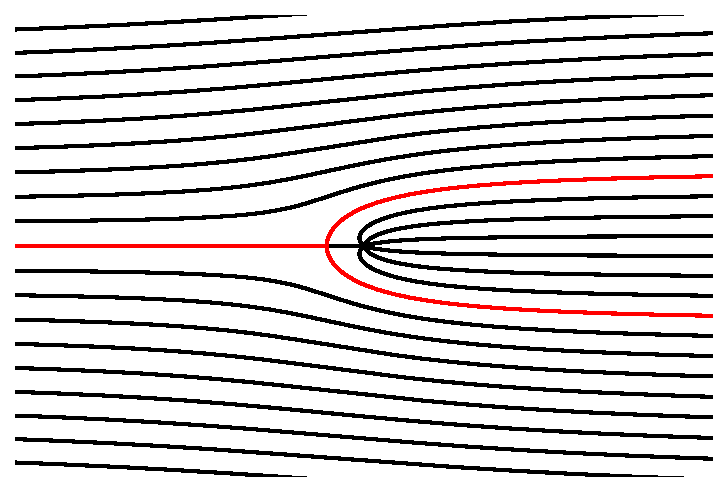
\includegraphics[width=0.7\linewidth]{Figures/Chapter4/fig_uniform_source}
\caption{Streamlines for a flow that includes both uniform flow and a line source.}
\label{fig_uniform_source}
\end{figure}


% SECTION 4.1.3 - METHOD OF IMAGES

\subsection{Method of Images}
\label{sec_images}

Consider a single line vortex, but we'll modify the flow in two ways:  first, by moving it to a new position $z_0 = d$ along the $x$ axis, and secondly by putting a wall at $x=0$, effectively having the fluid in the domain $x>0$ only.  This is shown in Figure \ref{fig_mirror_wall}.  Now, the first adjustment is easy to make, since moving the line vortex location just means shifting the origin in the opposite direction; in general, a line vortex at a location $z_0 = x_0 + iy_0$ in the complex plane is given by
\begin{equation}
\label{eq_line_vortex_z0}
w(z) = -\frac{i\Gamma}{2\pi} \ln (z-z_0).
\end{equation}

\begin{figure}
\centering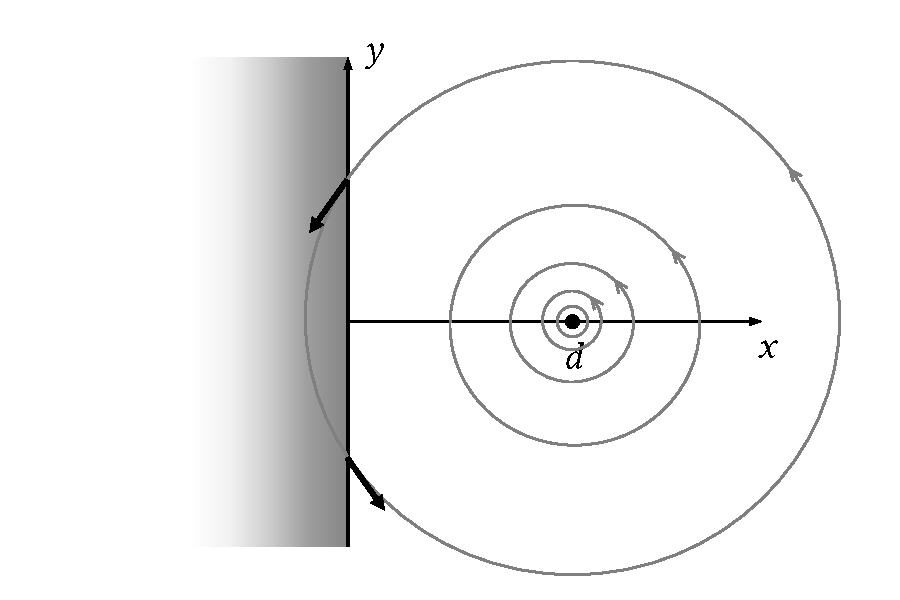
\includegraphics[width=0.75\linewidth]{Figures/Chapter4/fig_mirror_wall}
\caption{A line vortex a distance $d$ from a wall.}
\label{fig_mirror_wall}
\end{figure}

What about the wall?  That's a little trickier, since it's apparent that the flow given in equation (\ref{eq_line_vortex_z0}) doesn't satisfy the boundary conditions -- we need the flow to slip along the wall.  That means we require our flow at $x=0$ to be along the $y$ direction only, so that
\[
u(0, y) = 0.
\]
As shown in Figure  \ref{fig_mirror_wall}, the flow is tangent to the streamlines, and doesn't point just along $y$ at the wall.  In fact, it looks like the fluid is either flowing \emph{into} the wall or \emph{out of} the wall, which doesn't make much sense physically.  How can we adjust our complex potential to satisfy the boundary condition?

Well, never mind for a moment.  Instead, consider a completely \emph{different} problem:  two vortexes, one at $z = d$ as above, and one at $z = -d$; there's no wall in this problem.  The second vortex will have the same strength as the first, but will go in the opposite direction:  $\Gamma_2 = - \Gamma_1$; see Figure \ref{fig_mirror_image}.  Since complex potentials add together, it's simple to write down $w(z)$ for this new flow:
\[
w(z) = -\frac{i\Gamma}{2\pi} \ln (z-d) + \frac{i\Gamma}{2\pi} \ln (z+d)
\]
(notice the plus sign -- the second term is for the vortex that rotates in the opposite sense as the first).  We can simplify this a bit using log rules to get
\begin{equation}
\label{eq_mirror_vortex}
w(z) = -\frac{i\Gamma}{2\pi} \ln \left( \frac{z - d}{z+d} \right).
\end{equation}

Now, \emph{this} flow \emph{does} satisfy the boundary condition -- the two flows from each vortex combine at the wall and the $x$ components of the velocity end up cancelling, giving components along the $y$ direction only.  In other words, this flow slips along the boundary; you can prove this mathematically if you want by trying Problem \ref{prob_mirror_bc}.

\begin{figure}
\centering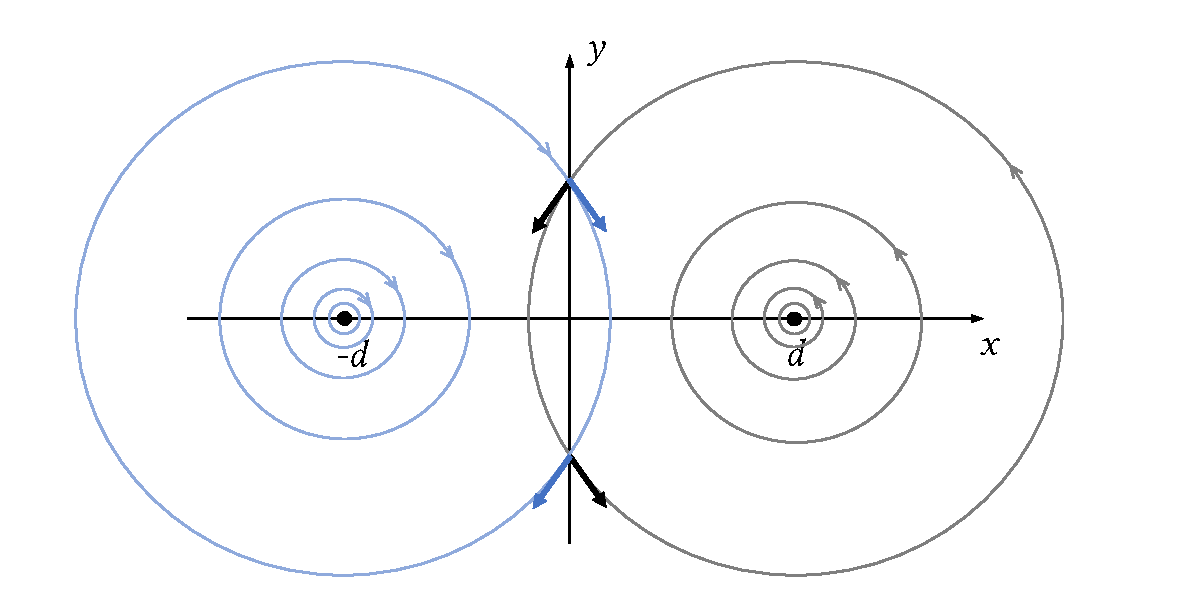
\includegraphics[width=\linewidth]{Figures/Chapter4/fig_mirror_image}
\caption{Two line vortexes combine to create a flow that slips along the wall.}
\label{fig_mirror_image}
\end{figure}

By adding a second vortex, we've satisfied the boundary conditions of the original problem; this is a technique called method of images, which you might know from electrostatics.  Of course, in the original problem, we had only \emph{one} vortex, not two -- but that's okay, since our second vortex is covered up by the wall.  It's not really there, and our solution is only good for the domain $x>0$.  

Method of images works because our fluid satisfies Laplace's equation, and solutions to Laplace's equation are \emph{unique}: if a complex potential is a solution to Laplace's equation \emph{and} satisfies the boundary conditions of the problem, then it's \emph{the} solution.\footnote{Griffiths has an excellent discussion of uniqueness theorems and Laplace's equation in \emph{Introduction to Electrodynamics}, 4th edition, Chapter 3; as usual there's much more to say about the matter.}

One more thing before we move on.  What does the flow in $x>0$ actually look like?  Figure \ref{fig_mirror_image} gives streamlines for each vortex superimposed, not combined properly.  To find the streamlines, we need the stream function,
\[
\psi = \operatorname{Im}(w).
\]
As I mentioned above, it's not always easy to find the imaginary part of the complex potential, particularly when logarithms are involved.  I'll walk you through a general method for doing so, and we'll start with the polar form of the complex number $z$:
\[
z = s e^{i\phi}.
\]
Here, $s$ is often called the \emph{modulus}, and is the complex absolute value of $z$,
\[
s = |z| = \sqrt{z^*z},
\]
and $\phi$ is called the argument.  Now, if we just have the logarithm of a complex number, that's easy enough to split into real and imaginary parts, and we've already seen the reverse of it in Example \ref{ex_line_vortex_w}:
\[
\ln z = \ln s + i\phi.
\]
Note that the real part of $\ln z$ is the logarithm of the modulus $s$ and the imaginary part is the argument $\phi$.  Careful, though -- in fact, I could add a multiple of $2\pi$ to $\phi$ and still get the same $\ln z$, so there's actually an infinite number of possibilities for the imaginary part of $\ln z$.  Writing it as I did means $\ln z$ is called the \emph{principle value.} This is something we won't have to worry about much, but I wanted to mention it for completeness. 

If we have something more complicated, say the logarithm of a complex function $f(z)$, the idea is the same,
\[
\ln \left[ f(z) \right] = \ln \left| f(z) \right| + i \operatorname{Arg} \left[ f(z) \right].
\]

Now, it might not be simple to find the argument of the function $f(z)$ -- you'll have to split it into its real and imaginary parts, 
\[
f(z) = A(x, y) + iB(x, y),
\]
and then find the argument from
\[
\operatorname{Arg}\left[ f(z) \right] = \operatorname{Arg}\left[ A(x, y) + iB(x, y) \right] = \tan^{-1} \left[ \frac{B(x,y)}{A(x,y)} \right].
\]
Things can once again get complicated in dealing with the arctan function, but luckily we won't have to worry about this much either.  The modulus at least is normally not a problem, since
\begin{equation}
\left| f(z) \right| = \sqrt{ f^*(z) f(z) }.
\end{equation}

In the case of the vortex beside the wall, we can now write
\[
w(z) = -\frac{i\Gamma}{2\pi} \ln \left( \frac{z - d}{z+d} \right) = -\frac{i\Gamma}{2\pi} \left[ \ln \left| \frac{z-d}{z+d} \right| + i \operatorname{Arg} \left( \frac{z-d}{z+d} \right) \right]
\]
or
\[
w(z) = \frac{\Gamma}{2\pi}\operatorname{Arg} \left( \frac{z-d}{z+d} \right) - i \frac{\Gamma}{2\pi} \ln \left| \frac{z - d}{z+d} \right|,
\]
and we can identify the stream function as the imaginary part,
\begin{equation}
\psi(x, y) = \frac{\Gamma}{2\pi} \ln \left| \frac{z - d}{z+d} \right|.
\end{equation}
Careful, though -- there are still complex numbers $z$ in that equation for $\psi$, which should be a real function.  However, because the complex absolute value is there, it's guaranteed to be real -- if you work it out (it's a bit of algebra but not too hard), you get
\begin{equation}
\psi(x, y) = -\frac{\Gamma}{2\pi} \ln \sqrt{ \frac{x^2 + y^2 - 2xd + d^2}{x^2 + y^2 + 2xd + d^2} }.
\end{equation}
From the stream function you can plot the streamlines of the flow as shown in Figure \ref{fig_vortex_wall}; notice that one streamline lies directly along the wall.

\begin{figure}
\centering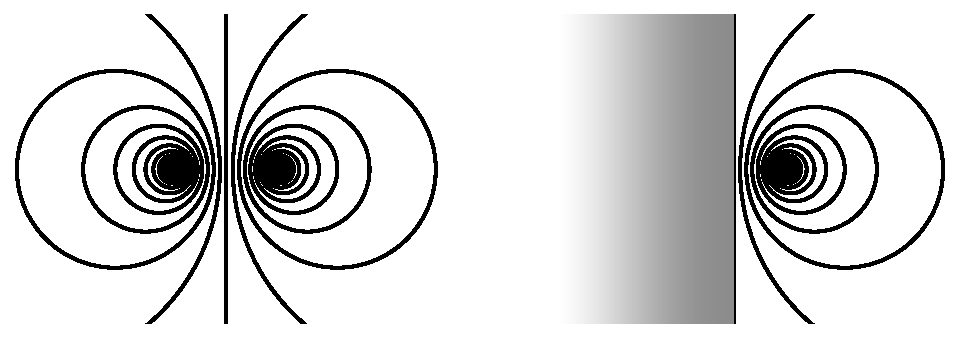
\includegraphics[width=0.9\linewidth]{Figures/Chapter4/fig_vortex_wall}
\caption{The streamlines for a line vortex a distance $d$ from a wall.  The left side shows both vortexes, while the right side shows just the real vortex beside the wall.}
\label{fig_vortex_wall}
\end{figure}


% SECTION 4.1.4 - THE CIRCLE THEOREM

\subsection{The Circle Theorem}

Take a close look at Figure \ref{fig_vortex_wall} -- although the circular streamlines are no longer \emph{concentric}, they are still circular.  That suggests that this complex potential can also work for a line vortex within a \emph{circular} boundary (say, a cylindrical bucket filled with fluid) -- as long as the boundary matches one of the streamlines, our boundary condition will be satisfied and the fluid will slip along the circular wall.

Consider the situation shown in Figure \ref{fig_circular_boundary}.  We'll put the origin of our coordinate system at the centre of the cylindrical bucket (of radius $a$) and orient the $x$ axis so that the line vortex of strength $\Gamma$ is located on it at $x = c_1$.  To ensure a streamline matches the boundary of the cylinder, we'll need a mirror image of the vortex (with opposite circulation $-\Gamma$) on the $x$ axis -- outside the cylinder.  The question is \emph{where} do we put it?

\begin{figure}
\centering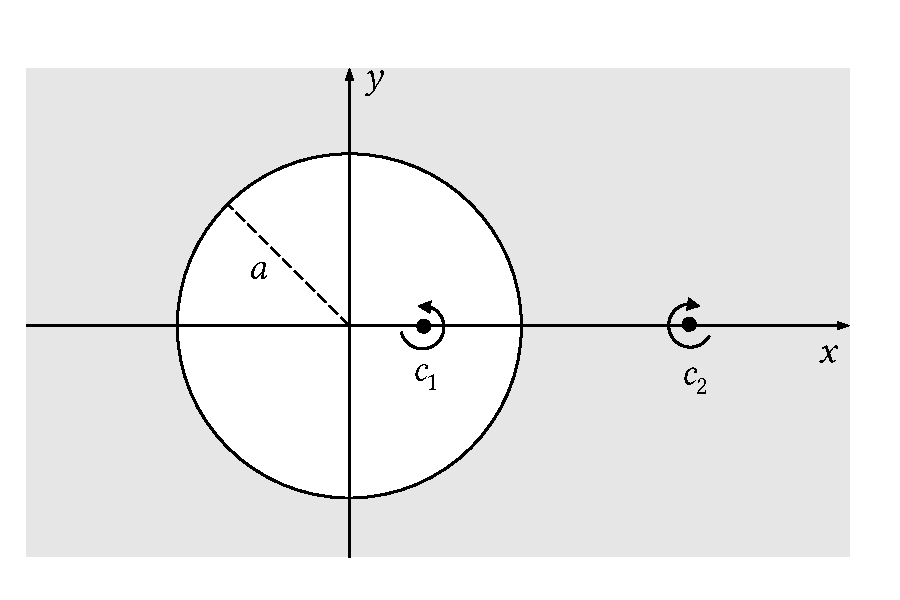
\includegraphics[width=0.75\linewidth]{Figures/Chapter4/fig_circular_boundary}
\caption{A line vortex in a circular bucket can be modelled with a mirror image outside the bucket.}
\label{fig_circular_boundary}
\end{figure}

Take a look at the circles on the left side of Figure \ref{fig_vortex_wall} again -- they're a well-known system called \emph{coaxal circles}.  The members of a coaxal system are described by the equation
\begin{equation}
\label{eq_coaxal_circles}
x^2 + y^2 + 2\lambda x + k = 0,
\end{equation}
with different values of $\lambda$ giving different circles.  These two sets of circles have \emph{limiting points} at $x = \pm \sqrt{k}$ -- that's where they converge to a circle of radius zero.  In our problem here, the positions of the two line vortexes at $x=c_1$ and $x=c_2$ would be the limiting points. From equation (\ref{eq_coaxal_circles}) you can derive a relationship between the radius $a$ of one of the circles and the two limiting points; it turns out to be
\[
a^2 = c_1 c_2.
\]
If we have a vortex at $x=c_1$ inside the cylinder, placing a mirror vortex at 
\begin{equation}
c_2 = \frac{a^2}{c_1}
\end{equation}
will give streamlines that match the boundary.  The complex potential of a vortex in a cylindrical bucket a distance $c$ from the centre is therefore
\begin{equation}
w(z) = -\frac{i\Gamma}{2\pi} \ln (z-c) + \frac{i\Gamma}{2\pi} \ln (z-a^2/c)
\end{equation}
(I've dropped the subscript ``1'' from $c$ since we don't need $c_2$ anymore), and the streamlines are shown in Figure \ref{fig_vortex_cylinder}.

%\begin{figure}
%\centering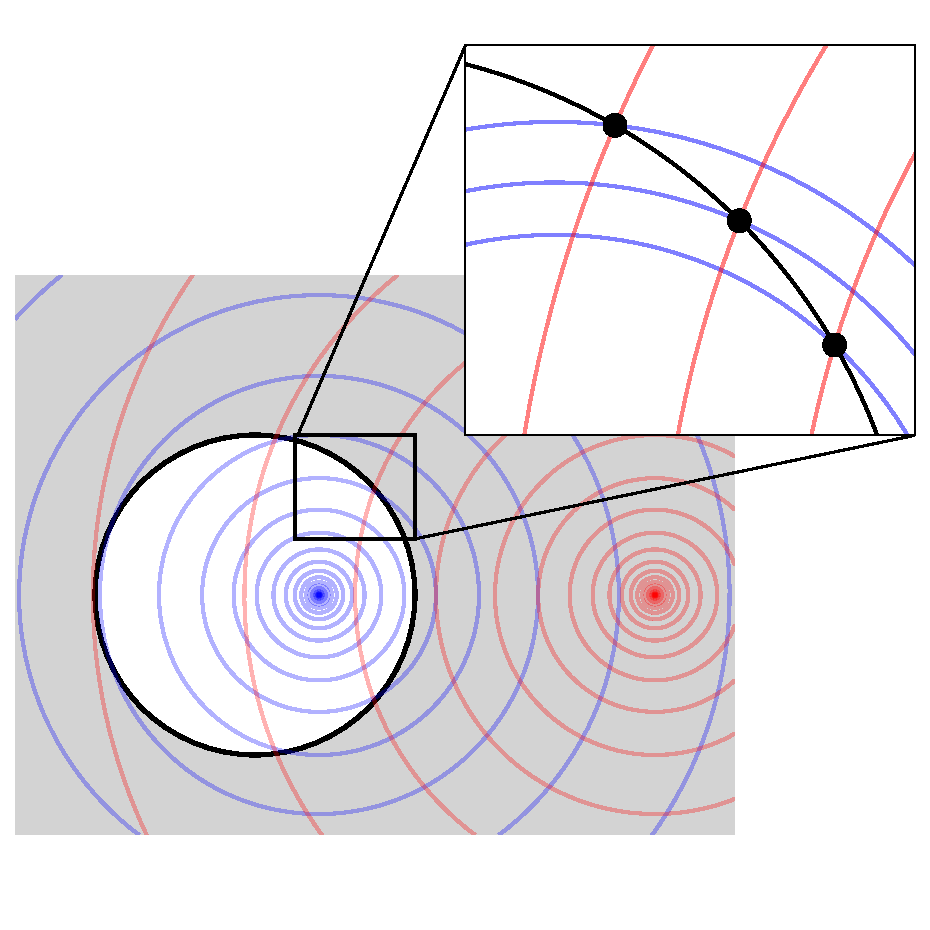
\includegraphics[width=0.75\linewidth]{Figures/Chapter4/fig_circular_inset}
%\caption{The streamlines of the two vortexes combine to give a streamlines that exactly matches the cylinder.}
%\label{fig_circular_inset}
%\end{figure}

\begin{figure}
\centering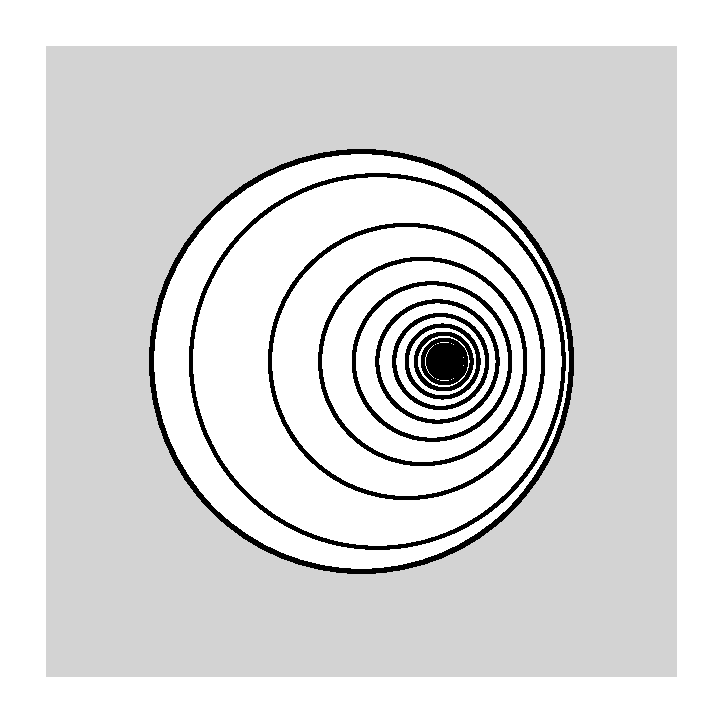
\includegraphics[width=0.5\linewidth]{Figures/Chapter4/fig_vortex_cylinder}
\caption{The streamlines of a line vortex within a circular cylinder.}
\label{fig_vortex_cylinder}
\end{figure}

The idea of placing a vortex in a flow to get a circular streamline is very general -- and powerful.  The Milne-Thompson Circle Theorem gives us a way to add a circular streamline to any irrotational, incompressible flow, and is given by the following:
\begin{theorem}[Milne-Thompson Circle Theorem]
Consider a flow described by the complex potential
\[
w = f(z),
\]
and any singularities of $f(z)$ (in other words, where it goes to infinity) occur in the region $|z| > a$.  Then the new complex potential
\begin{equation}
w = f(z) + f^*(a^2 / z^*)
\end{equation}
describes a flow that has the same singularities as $f(z)$ in $|z| > a$ \emph{and} has the circle $|z| = a$ as a streamline.
\end{theorem}

This is straightforward to prove.  The circle $|z| = a$ can be written as
\[
|z|^2 = z^* z = a^2,
\]
or
\[
z^* = \frac{a^2}{z}.
\]
That means that, on the circle itself,
\[
w = f(z) + f^*(a^2/z^*) = f(z) + f^*(z).
\]
But the function $f(z) + f^*(z)$ is a \emph{real} function; suppose we write $f(z) = A(x, y) + iB(x, y)$, in which case it's easy to see that 
\[
f(z) + f^*(z) = A(x, y) + iB(x,y) + A(x, y) - iB(x, y) = 2A(x, y),
\]
and the imaginary part has cancelled. If $w(z)$ is a \emph{real} function on the circle, then it's imaginary component must be zero:
\[
\psi(x, y) = \operatorname{Im}(w) = 0.
\]
Never mind the zero -- the important thing is to see that $\psi$ is \emph{constant} along the circle.  That means the circle is a streamline!

What about the singularity part?  Well, any point that is originally outside the circle in $f(z)$ actually ends up \emph{inside} the circle in $f^*(a^2/z^*)$, so no new singularities outside $|z| = a$ are created -- that means the new flow has the same singularities as the original flow.

%
% SECTION 4.2 - FLOW PAST OBJECTS
%

\section{Flow Past Objects}



% SECTION 4.2.1 - FLOW PAST A CYLINDER

\subsection{Flow Past a Cylinder}

As a simple example of the Circle Theorem, consider starting with uniform flow with angle $\alpha = 0$, given by
\[
w(z) = Uz.
\]
Using the Circle Theorem we get
\[
w(z) = Uz + \left[ U \frac{a^2}{z^*} \right]^*
\]
or
\begin{equation}
w(z) = U \left( z + \frac{a^2}{z} \right).
\end{equation}
This is the complex potential for a flow that is uniform at infinity but has a circular streamline centred at the origin with radius $a$; see Figure \ref{fig_uniform_circle}. The streamlines outside the circular streamline might look familiar if you recall Section \ref{sec_cylinder}, and we'll examine them closely in a moment.  But what about the streamlines interior to the circle?  They're similar to the streamlines for a \emph{doublet} flow, in which $w \propto z^{-1}$, but that doesn't really matter -- in fact, if we ``cover up'' the fluid interior to $|z| = a$ with, say, a circular cylinder, then what we've done is find the complex potential for flow around that cylinder.

\begin{figure}
\centering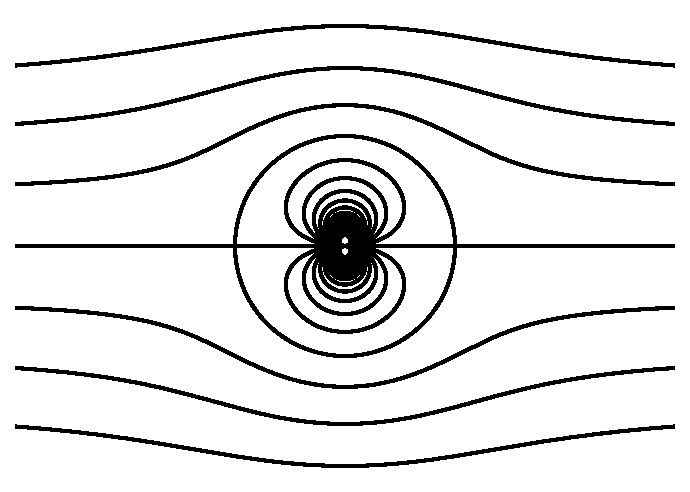
\includegraphics[width=0.7\linewidth]{Figures/Chapter4/fig_uniform_circle}
\caption{The streamlines for the flow generated by applying the Circle Theorem to a uniform flow.}
\label{fig_uniform_circle}
\end{figure}

Does our solution match the one we found earlier in Section \ref{sec_cylinder}?  We can find the velocity potential and stream function easily enough (see Problem \ref{prob_circlular_cylinder}); they are
\begin{equation}
\varphi(s, \phi) = U \left( s + \frac{a^2}{s} \right) \cos\phi
\end{equation}
and
\begin{equation}
\psi(s, \phi) = U \left( s - \frac{a^2}{s} \right) \sin\phi.
\end{equation}
We can also find the velocity of the flow, either from the potential or stream function, or from the derivative of the complex potential directly using equation (\ref{eq_w_deriv}); either way, we get
\begin{equation}
u_s(s, \phi) = U \left( 1 - \frac{a^2}{s^2} \right) \cos\phi
\end{equation}
and
\begin{equation}
u_\phi(s, \phi) = U \left( 1 + \frac{a^2}{s^2} \right) \sin\phi.
\end{equation}
These do indeed match the flow we found earlier -- by much more laborious means (solving Laplace's equation).  It's hard to overstate just how powerful the Circle Theorem can be; we found in a few lines what took us four pages of solving a partial differential equation before.

But we can do more in this case.  It's trivial to add an angle $\alpha$ to the uniform flow, for example; in that case we start with the complex potential
\[
w(z) = Uz e^{-i\alpha}
\]
and get, using the Circle Theorem,
\begin{equation}
w(z) = U \left( ze^{-i\alpha} + \frac{a^2}{z}e^{i\alpha} \right).
\end{equation}
We could also add a line vortex, placed at the origin, to our flow.  This wouldn't change the fact that there's a circular streamline at $|z| = a$, since the line vortex has circular streamlines, but would change the flow $u_\phi$ at the surface of the cylinder -- in effect, we're adding \emph{circulation} to the flow, as we'll see.  Remember, complex potentials add together, so the flow with a line vortex is simply
\begin{equation}
\label{eq_uniform_circle}
w(z) = U \left( ze^{-i\alpha} + \frac{a^2}{z}e^{i\alpha} \right) - \frac{i\Gamma}{2\pi} \ln z.
\end{equation}

\begin{figure}
\centering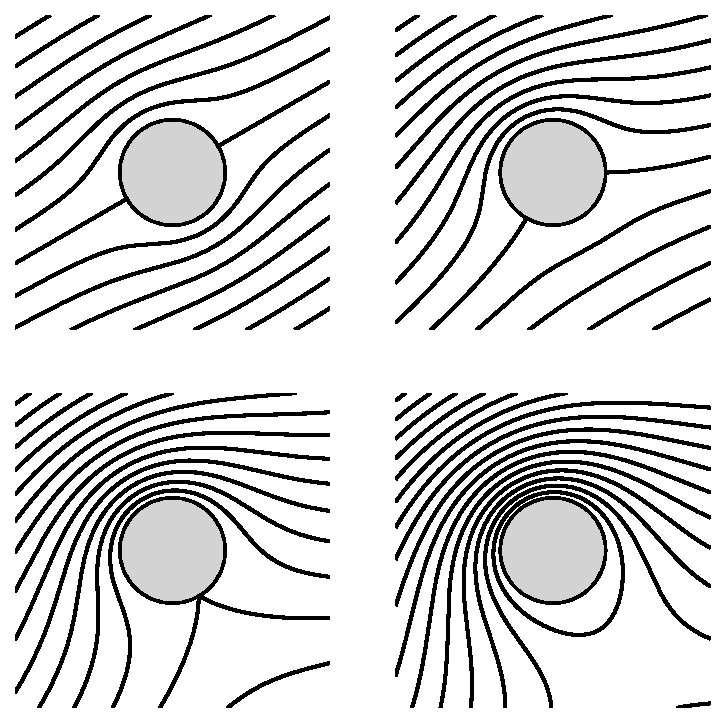
\includegraphics[width=0.75\linewidth]{Figures/Chapter4/fig_cylinder_circ}
\caption{Streamlines for flow around a circular cylinder at an angle $\alpha = \pi/6$.  Upper left: circulation $\Gamma = 0$.  Upper right: circulation $\Gamma = -2\pi Ua$.  Lower left: circulation $\Gamma = -4\pi Ua$.  Lower right: circulation $\Gamma = -6\pi Ua$.}
\label{fig_cylinder_circ}
\end{figure}

Streamlines with circulation in the flow are shown in Figure \ref{fig_cylinder_circ}.  Something interesting happens as the circulation $\Gamma$ increases:  notice that the two stagnation points, normally at opposite ends of the cylinder, come closer together as the circulation increases, until 
\[
\Gamma = \pm 4\pi U a,
\]
when they combine to form just one stagnation point.  If the circulation is greater than this, they disappear completely -- we now have fluid circulating completely around the cylinder, as you can see by the streamlines in the lower right part of Figure \ref{fig_cylinder_circ} (note that the circulation is negative in the Figure, so that the fluid circulates clockwise around the cylinder; we'll see why I chose this shortly).  You can explore this flow more in Problem \ref{prob_circlular_cylinder}.

Back in Problem \ref{prob_force1} you may have calculated the force of the fluid on a circular cylinder for flow without circulation -- it turned out to be zero, a somewhat surprising result called d'Alembert's paradox.  Because we're dealing with ideal fluids and the flow is symmetric, the fluid is unable to push on the cylinder.  However, this result changes when circulation is added to the flow.  Problem \ref{prob_force2} can walk you through the details of the calculation, but nothing changes for the $x$ component of force -- the fluid still doesn't push on the cylinder in the direction of the oncoming flow -- but there \emph{is} a force in the $y$ direction, perpendicular to the uniform flow:
\begin{equation}
\label{eq_force1}
F_y = -\rho U \Gamma.
\end{equation}
This force is due entirely to the circulation around the cylinder, and if $\Gamma$ is negative, as the examples in Figure \ref{fig_cylinder_circ} show, then the force is upward:  the fluid provides \emph{lift} on the cylinder.  Of course, the wings of an airplane aren't at all circular in cross section, but this essential idea -- that circulation around the object is necessary for lift -- will return when we discuss proper aerofoils.



% SECTION 4.2.2 - CONFORMAL MAPPING

\subsection{Conformal Mapping}

Suppose we have some general complex potential $w(z) = \varphi + i\psi$.  Our goal is to create a \emph{mapping} or \emph{transformation} between the complex plane $z = x+iy$ and a second complex plane, which I'll write with capital letters: $Z = X + iY$.  We'll perform this transformation with the function $f(z)$ such that
\begin{equation}
Z = f(z).
\end{equation}
We'll assume $f(z)$ is an \emph{analytic} complex function, meaning it's differentiable, and that it has an inverse given by
\begin{equation}
z = F(Z)
\end{equation}
(and $F(Z)$ is also an analytic function).

The complex potential is transformed as well -- in the $Z$ complex plane it takes on the form
\begin{equation}
W(Z) = w[F(Z)].
\end{equation}
Now, we can split $W(Z)$ into it's real and imaginary parts,
\begin{equation}
W(Z) = \Phi(X, Y) + i\Psi(X, Y).
\end{equation}
Here's the amazing thing:  because $W$ will be an analytic function of $Z$, $\Phi$ and $\Psi$ will satisfy the Cauchy-Riemann conditions (equation \ref{eq_cauchy_riemann}), and therefore
\begin{equation}
\U(X, Y) = \dfdx{\Phi}{X} = \dfdx{\Psi}{Y} \quad \text{and} \quad \V(X, Y) = \dfdx{\Phi}{Y} = -\dfdx{\Psi}{X}
\end{equation}
represent a possible fluid flow -- that is, the velocity  $\U \, \unit{X} +  \V \, \unit{Y}$ is an irrotational, incompressible flow that satisfies Laplace's equation.

This might seem like a lot to take in at first, but our goal is to use a transformation to map our flow around a circular cylinder to other possible shapes -- including, eventually, a realistic wing shape.  Before we get there, though, let's take a look at a simple example.



\begin{example}[A Simple Conformal Map]
\label{ex_conformal_map}
Consider the map
\[
Z = f(z) = \frac{z^2}{5} + 2,
\]
which has the inverse 
\[
z = F(Z) = \sqrt{5(Z-2)}.
\]
We'll start with the complex potential for uniform flow, $w(z) = Uz$; the left side of Figure \ref{fig_conformal_map} shows the streamlines (blue) as well as lines of constant velocity potential (red).  For uniform flow, these lines are straight and meet at right angles.

Under the map, the complex potential in the $Z$ complex plane becomes
\[
W(Z) = w[F(Z)] = U\sqrt{5(Z-2)};
\]
streamlines for this transformed complex potential are shown on the right panel of Figure \ref{fig_conformal_map}.  The original streamlines are mapped to new streamlines (and similarly for the lines of constant $\varphi$), and are no longer straight -- but notice that they do still cross at right angles.  This is why the mapping is called conformal -- the transformation preserves local angles.

Suppose we look at just one point in the $z$ complex plane, say
\[
z_0 = 1 + i.
\]
The complex potential at that point is $w(z_0) = U(1+i)$.  In the $Z$ complex plane, $z_0$ is mapped to
\[
Z_0 = \frac{2i}{5} + 2,
\]
but the complex potential $W(Z_0)$ has the same value as $w(z_0)$:
\[
W(Z_0) = U\sqrt{5(2i/5 + 2 - 2)} = U\sqrt{2i} = U(1+i).
\]

\end{example}

\begin{figure}
\centering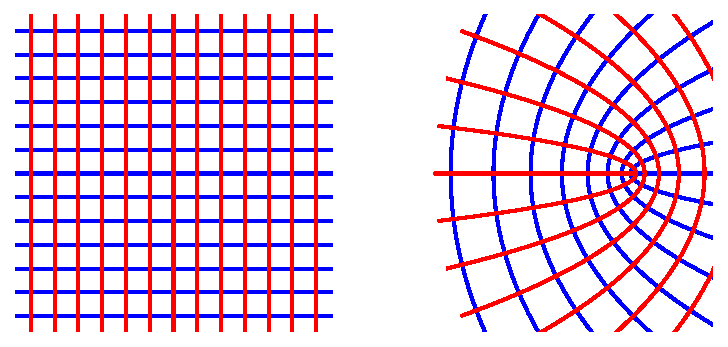
\includegraphics[width=0.75\linewidth]{Figures/Chapter4/fig_conformal_map}
\caption{The effect of the conformal map $f(z) = z^2/5 + 2$ on uniform flow.  The blue lines are the streamlines $\psi = $ constant and the red lines are lines of constant velocity potential $\varphi$.  Left: the original uniform flow, $w(z) = Uz$, in the $z$ complex plane.  Right: the flow under the conformal map $W(Z)$ in the $Z$ complex plane.}
\label{fig_conformal_map}
\end{figure}


When choosing a particular map, there are two things to be careful about.  First, consider the derivative of $W(Z)$.  Writing it as $W(Z) = w(z)$ where $z = F(Z)$, we can use the chain rule to get
\[
\frac{dW}{dZ} = \frac{dw}{dz}\frac{dz}{dZ}.
\]
But recall that $dw/dz = u - iv$, so this says
\begin{equation}
\label{eq_UV}
\U - i\V = \frac{u - iv}{dZ/dz} = \frac{u - iv}{f'(z)},
\end{equation}
using $Z = f(z)$.  If we want the streamlines in the new $Z$ complex plane to match the original streamlines in the $z$ plane at infinity -- far away from the object the fluid is flowing past -- then we'll need
\begin{equation}
f'(z) \to 1 \quad \text{as} \quad |Z| \to \infty.
\end{equation}

The second thing is about the conformal nature of the map.  Normally, local angles are preserved, as we saw in Example \ref{ex_conformal_map}.  However, this is only true if the mapping function $f(z)$ has a non-vanishing first derivative everywhere.  At points where the first derivative is zero, though, the angle changes; in general, the local angle is multiplied by $n$, where $n$ is the order of the first non-vanishing derivative of $f(z)$.  


% SECTION 4.2.4 - FLOW PAST AN ELLIPTICAL CYLINDER

\subsection{Flow Past an Elliptical Cylinder}

Let's try the following transformation:
\begin{equation}
Z = f(z) = z + \frac{c^2}{z},
\end{equation}
where $c$ is a constant.  This is called the \emph{Joukowski transformation}, and was important in the development of the theory of aerodynamics.  Note that the derivative is
\[
f'(z) = 1 - \frac{c^2}{z^2},
\]
so $f'(z) \to 1$ as $|z| \to \infty$; this mapping won't affect the flow far away from the object.  Also note that the first derivative is non-zero almost everywhere, so local angles will be preserved.  However, something interesting happens at $z = \pm c$ -- at that point the first derivative becomes zero, and the first non-vanishing derivative is the \emph{second}.  This means at those points local angles will be \emph{doubled}.

We'll need the inverse of the Joukowski transformation as well; it is given by
\begin{equation}
\label{eq_inverse_jt}
z = \frac{1}{2}Z \pm \sqrt{\frac{1}{4} Z^2 - c^2}.
\end{equation}
Note that, except at the points $Z = \pm 2c$, this inverse is \emph{multivalued}.  In the language of complex analysis, we would say that $Z = \pm 2c$ are \emph{branch points}, and we could cut the plane between them to ensure the inverse is single-valued.  However, in practice, we'll only need the positive root; it turns out that the negative root maps points in the $Z$ complex plane to points within a circle of radius $c$ on the $z$ complex plane, while the positive root maps them to points outside that circle.  Since we're studying fluid flow around objects, there won't be any fluid within that radius anyway -- the object itself will be there.

\begin{figure}
\centering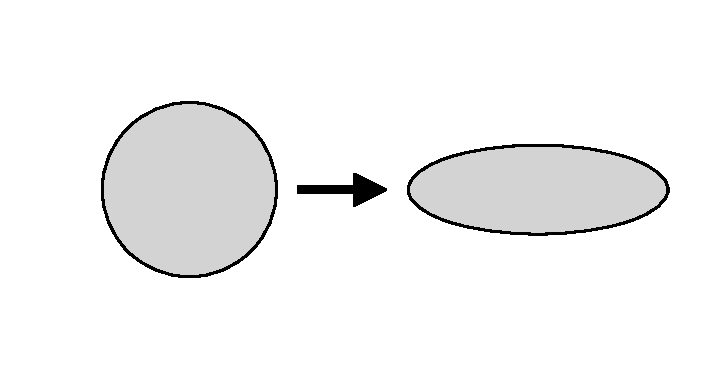
\includegraphics[width=0.75\linewidth]{Figures/Chapter4/fig_jt_ellipse}
\caption{The Joukowski transformation takes a circle in the $z$ complex place to an ellipse in the $Z$ complex plane.  Here the parameter $c = 0.7$.}
\label{fig_jt_ellipse}
\end{figure}

What does the Joulowski transform actually do?  Consider its affect on a circle of radius $a$ in the complex $z$ plane, which is given by
\[
z = a e^{i\phi}.
\]
Applying the transformation leads to 
\[
Z = z + \frac{c^2}{z} = ae^{i\phi} + \frac{c^2}{a} e^{-i\phi}.
\]
This might not look familiar, but with a bit of work we can see what it describes.  Write $Z = X + iY$ and $e^{i\phi} = \cos\phi + i\sin\phi$ and separate $Z$ into its real and imaginary components:
\[
X + iY = \left( a + \frac{c^2}{a} \right) \cos \phi + i \left( a - \frac{c^2}{a} \right) \sin \phi.
\]
Now take the complex conjugate of both sides and rearrange to get
\begin{equation}
\label{eq_ellipse}
\frac{X^2}{(a + c^2/a)^2} + \frac{Y^2}{(a - c^2/a)^2} = 1.
\end{equation}
This is the equation of an ellipse with semimajor axis $a + c^2/a$ and semiminor axis $a - c^2/a$. The shape of the ellipse is controlled by the parameter $c$, so that as $c \to a$, the ellipse gets flatter and flatter.  Figure \ref{fig_jt_ellipse} shows this Joukowski transformation.

To see what the flow around the ellipse looks like, we start with the flow around a circular cylinder of radius $a$ -- including the angle and circulation, as given by equation (\ref{eq_uniform_circle}) -- and use the inverse Joukowski transformation (equation \ref{eq_inverse_jt}) to replace all the $z$s with $Z$s. After a bit of rearranging, the complex potential around an elliptical cylinder is given by
\begin{multline}
\label{eq_ellipse_w}
W(Z) = Ue^{-i\alpha} \left( \frac{1}{2} Z + \sqrt{\frac{1}{4} Z^2 - c^2} \right) + Ue^{i\alpha} \frac{a^2}{c^2} \left( \frac{1}{2} Z - \sqrt{\frac{1}{4} Z^2 - c^2} \right) - \\ \frac{i\Gamma}{2\pi} \ln \left( \frac{1}{2} Z + \sqrt{\frac{1}{4} Z^2 - c^2} \right)
\end{multline}
To find the streamlines we have to extract the imaginary part of this very complicated complex potential.  Although possible, I'll leave it as an exercise for you to try; the streamlines themselves are shown in Figure \ref{fig_ellipse}. Luckily, producing the streamline plot with a computer is much easier than finding the streamlines by hand.

\begin{figure}
\centering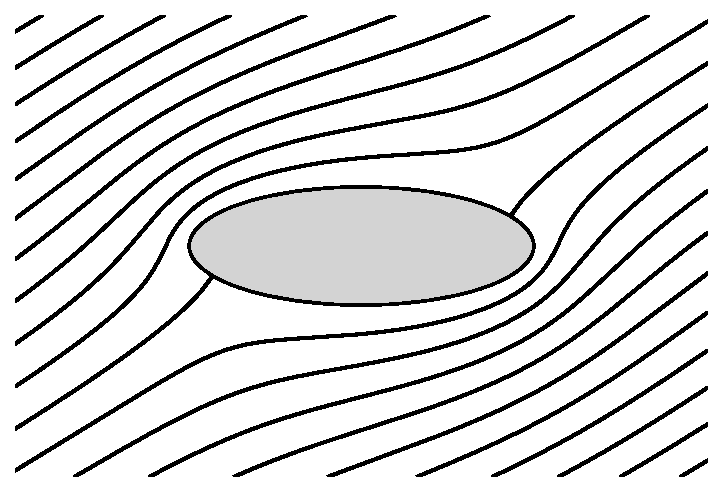
\includegraphics[width=0.7\linewidth]{Figures/Chapter4/fig_ellipse}
\caption{The streamlines for flow around an elliptical cylinder, with $c=0.7$, $\alpha = \pi/6$, and $\Gamma= 0$.}
\label{fig_ellipse}
\end{figure}


% SECTION 4.2.5 - FLOW PAST A FLAT PLATE

\subsection{Flow Past a Flat Plate}

The shape of the ellipse is dependent on the parameter $c$ in the Joukowski transformation, and if we let $c \to a$, so that the transformation is
\begin{equation}
Z = z + \frac{a^2}{z},
\end{equation}
the ellipse collapses to a flat plate.  Looking at equation (\ref{eq_ellipse}), we see that the semiminor axis goes to zero, while the semimajor axis becomes $2a$ -- so the plate has a total length of $4a$.  The flow in this case is shown in the left panel of Figure \ref{fig_flat_plate}.

Although it's difficult to see in that streamline plot, there are two points in the flow where the velocity goes to infinity -- there are two \emph{singularities}.  They occur at each edge of the plate, at $Z = \pm 2a$.  To investigate the velocity of the flow, we have to find the derivative $dW/dZ$, which can be lengthy and complicated.  To simplify things for a bit, suppose $\Gamma = 0$; letting $a=c$ in equation (\ref{eq_ellipse_w}) and taking the derivative, we get (with some simplification)
\[
\U - i\V = \frac{dW}{dZ} = U\cos \alpha - i \frac{U \sin \alpha \, Z}{\sqrt{Z^2 - 4a^2}}.
\]
You can see in the imaginary term that the denominator goes to zero as $Z \to \pm 2a$ -- so the $Y$ component of the velocity blows up there and we have a singularity in the flow.

\begin{figure}
\centering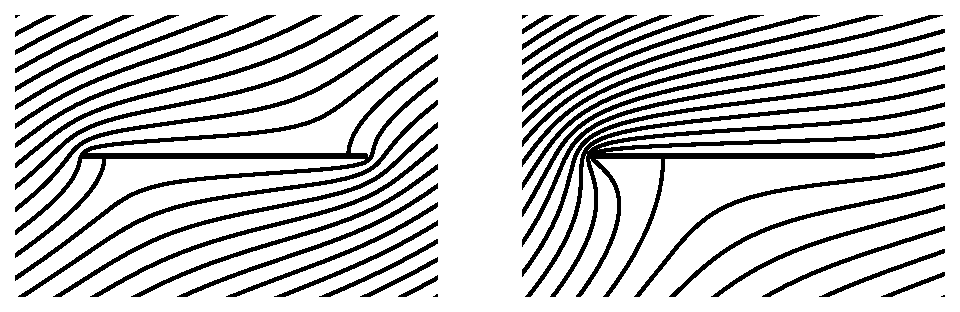
\includegraphics[width=\linewidth]{Figures/Chapter4/fig_flat_plate}
\caption{The streamlines for flow around a flat plate with angle $\alpha = \pi/6$.  Left: $\Gamma = 0$.  Right: $\Gamma= -4\pi Ua \sin\alpha$.}
\label{fig_flat_plate}
\end{figure}

Now, a singularity is not physical, so presumably in a real fluid flowing past a thin flat plate they would not exist.  One way to remove them is to set $\alpha = 0$, but that's not very general.  We can do better, but we need to resort to a bit of a trick to analyze this situation.  If we include the circulation term in equation (\ref{eq_ellipse_w}), the derivative gets even messier, so let's use equation (\ref{eq_UV}) to find the velocity components $\U$ and $\V$:
\begin{equation}
\label{eq_dwdz}
\U - i\V = \frac{dW}{dZ} = \frac{dw/dz}{f'(z)} = \frac{Ue^{-i\alpha} - U(a^2/z^2) e^{i\alpha} - i\Gamma/2\pi z}{1 - a^2/z^2}.
\end{equation}
Notice that the velocity goes to infinity at $z = \pm a$, which corresponds in the $Z$ complex plane to $Z = \pm 2a$ as we just found.  At this point, we should use the inverse Joukowski transformation, equation (\ref{eq_inverse_jt}), to replace all the $z$s with $Z$s, but it's not necessary as long as we're careful.

If you look at the velocity, you might notice that we can remove \emph{one} singularity from the flow by choosing just the right amount of circulation:  if 
\begin{equation}
\Gamma = -4\pi Ua \sin \alpha,
\end{equation}
then the numerator of equation (\ref{eq_dwdz}) goes to zero at $z = +a$ along with the denominator.  You can show that, in this case, the flow remains finite at $z = a$ and becomes (see Problem \ref{prob_flat_plate})
\begin{equation}
\U = U\cos\alpha \quad \text{and} \quad \V = 0 \quad \text{at} \quad Z = 2a.
\end{equation}
The flow with this choice is shown in the right hand panel of Figure \ref{fig_flat_plate}. We've removed the singularity at the right edge of the plate -- called the \emph{trailing edge} -- with an astute choice of circulation, but the singularity still exists at the \emph{leading edge}.  To fix that one, we'll have to do one more clever trick.




% SECTION 4.2.6 - FLOW PAST AN AEROFOIL

\subsection{Flow Past an Aerofoil}

The trick is simple -- we're going to hide the leading edge singularity \emph{inside} the object, where there is no fluid.  To do that, we'll shift the circle in the $z$ complex plane to the left by an amount $\lambda$; see the left panel of Figure \ref{fig_aerofoil} for how this looks. Note that we still want the circle to extend to $z=+a$ on the right side, so we'll also increase the radius of the circle to $a + \lambda$.  Even if $\lambda$ is a small value, $z=-a$ will be covered by the circle, and when transformed to the $Z$ complex plane, the point $Z = -2a$ will be covered by the object the circle is transformed into under the Joukowski transformation -- a classic aerofoil shape, as shown in the right panel of Figure \ref{fig_aerofoil}.

\begin{figure}
\centering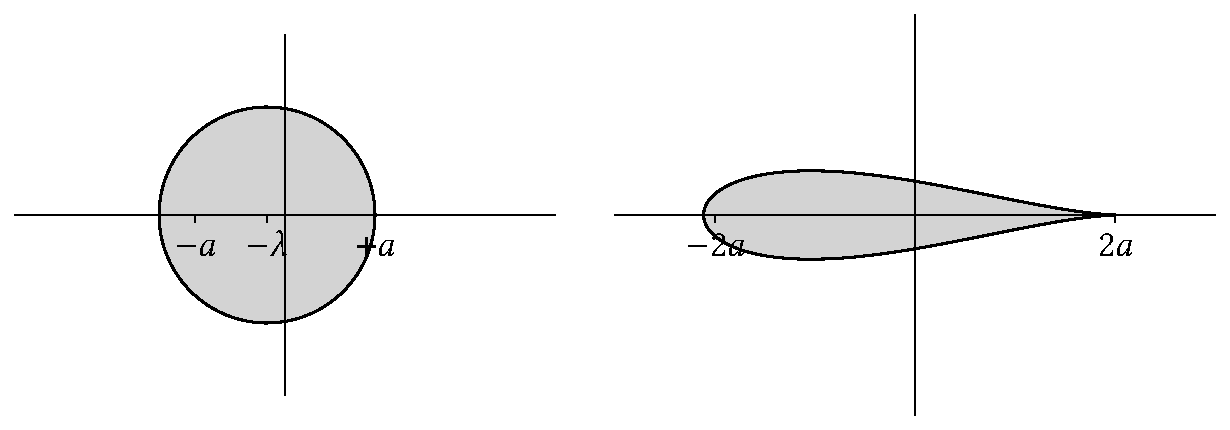
\includegraphics[width=\linewidth]{Figures/Chapter4/fig_aerofoil}
\caption{The Joulowski transformation takes the circle, shifted to the left by an amount $\lambda$, into an aerofoil shape.}
\label{fig_aerofoil}
\end{figure}

The complex potential around the shifted circle can be found by replacing $z$ with $z+\lambda$ and $a$ with $a+\lambda$, and it becomes
\begin{equation}
w(z) = U\left[ (z+\lambda) e^{-i\alpha} + \frac{(a+\lambda)^2}{z+\lambda} e^{i\alpha} \right] - \frac{i\Gamma}{2\pi} \ln (z+\lambda).
\end{equation}
As usual, to find the complex potential $W(Z)$ around the aerofoil, we replace $z$ with $Z$ using the inverse Joukowski transform, equation (\ref{eq_inverse_jt}).  Feel free to try that on your own.  But we can also examine the velocity of the flow around the aerofoil with the same trick we did above -- using equation (\ref{eq_UV}):
\begin{equation}
\U - i\V = \frac{dw/dz}{f'(z)} = \frac{ U e^{-i\alpha} - Ue^{i\alpha} (a+\lambda)^2 / (z+\lambda)^2 - i\Gamma / 2\pi(z+\lambda)}{1-a^2/z^2}
\end{equation}
From this equation, it looks like we still have singularities at $z=\pm a$ or $Z = \pm 2a$.  However, if we once again specify the circulation, we can remove the singularity at $z=+a$; we need to set 
\begin{equation}
\Gamma = -4\pi U (a + \lambda) \sin \alpha
\end{equation}
for the flow to remain finite there.  If the aerofoil is ``thin,'' so that $\lambda \ll a$, then $\Gamma$ reduces to that for the flat plate.  This value of the circulation is called the \emph{Kutta-Joukowski condition}, something we'll discuss in more depth momentarily.

What about the singularity at $z = -a$ or $Z = -2a$?  We don't have to worry about that one -- it's covered by the aerofoil, and so there is no fluid there.  Our trick worked, and as long as we have the right circulation, the flow is everywhere finite around the wing.  The streamlines are shown in Figure \ref{fig_aerofoil_stream}.

\begin{figure}
\centering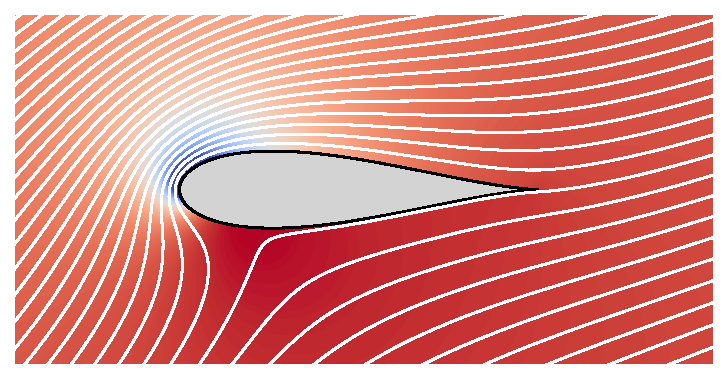
\includegraphics[width=\linewidth]{Figures/Chapter4/fig_aerofoil_stream}
\caption{The streamline and pressure of the flow around an aerofoil.  Here $\alpha = \pi/6$, $\Gamma = -4\pi U(a+\lambda) \sin \alpha$, and $\lambda = 0.2$.}
\label{fig_aerofoil_stream}
\end{figure}

Now that we have the velocity $[\U, \V]$ of the fluid around the aerofoil, we could in principle find the pressure from Bernoulli's principle -- we're still dealing with steady, irrotational flow, so $H$ is constant within the fluid, and we can write
\[
\frac{p_\infty}{\rho} + \frac{1}{2} U^2 = \frac{p(s, \phi)}{\rho} + \frac{1}{2} \vec{u}^2,
\]
calculate $\vec{u}^2 = \U^2 + \V^2$ and solve for the pressure $p(s, \phi)$.  As usual, that's a complicated procedure by hand, but easier with a computer, and Figure \ref{fig_aerofoil_stream} shows the pressure around the aerofoil.

Then, given the pressure, we could integrate around the aerofoil to find the force -- again, too complicated for us to do here.  But it \emph{is} possible to do using more advanced complex analysis techniques, and it turns out that, regardless of the shape of the object, the result is always the same:
\begin{equation}
\vec{F} = - \rho U \Gamma \, \unit{y},
\end{equation}
where the coordinate system is chosen such that the uniform flow far away is directed along the positive $x$ axis.  This is the same result as for a circular cylinder, equation (\ref{eq_force1}), and it's correct for the aerofoil as well.  This general result is called the \emph{Kutta-Joukowski theorem.}

That brings us finally to a classic fluid dynamics question:  how do airplanes fly?  The answer, of course, as anyone who has stuck their hand out the window of a moving car knows, is that the wing deflects the air downward, causing an upward force on the wing itself.  However, the Kutta-Joukowski condition and theorem give an alternative explanation.

We need two bits of information.  First, recall Kelvin's Circulation Theorem from Section \ref{sec_circulation}, which says that the circulation $\Gamma$ around a dyed, closed curve $C(t)$ in the fluid is constant.  And second, we know that for there to be a singularity-free flow around an aerofoil, there must be circulation $\Gamma = -4\pi Ua \sin \alpha$, and that this circulation is what provides upward lift on the aerofoil.  Consider, then, what happens as an airplane starts moving down the runway to take off -- see Figure \ref{fig_airplane}.

When the airplane is initially at rest, before starting takeoff (top panel), the circulation around the curve $C(t)$ is obviously \emph{zero} -- the wing and fluid are at rest.  Then the wing starts to move to the left, or, as in our reference frames above where the object is at rest, the fluid starts to move to the right.  For there to be no singularities in the flow, there must be circulation around the wing -- but the \emph{total} circulation is still zero from Kelvin's Circulation Theorem.  So there must be some \emph{additional} circulation within $C(t)$, and in the opposite sense to balance out.  This is called a \emph{starting vortex}, and is easily seen in real airplanes or even with some water, food colouring, and a plastic card, as shown in Figure \ref{fig_starting_vortex}.  Notice the vortex is counterclockwise, as expected.  Why does the airplane fly?  Because the circulation generated around the wing provides \emph{lift}.  As the airplane travels faster (so larger $U$), both the circulation and the lift force increase.

\begin{figure}
\centering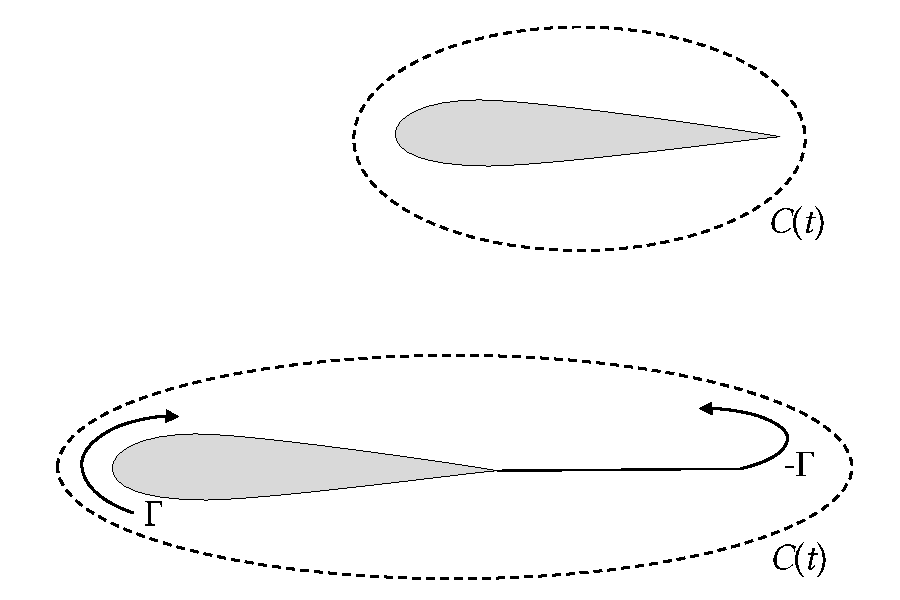
\includegraphics[width=0.8\linewidth]{Figures/Chapter4/fig_airplane}
\caption{An airplane taking off induces a starting vortex.}
\label{fig_airplane}
\end{figure}

\begin{figure}
\centering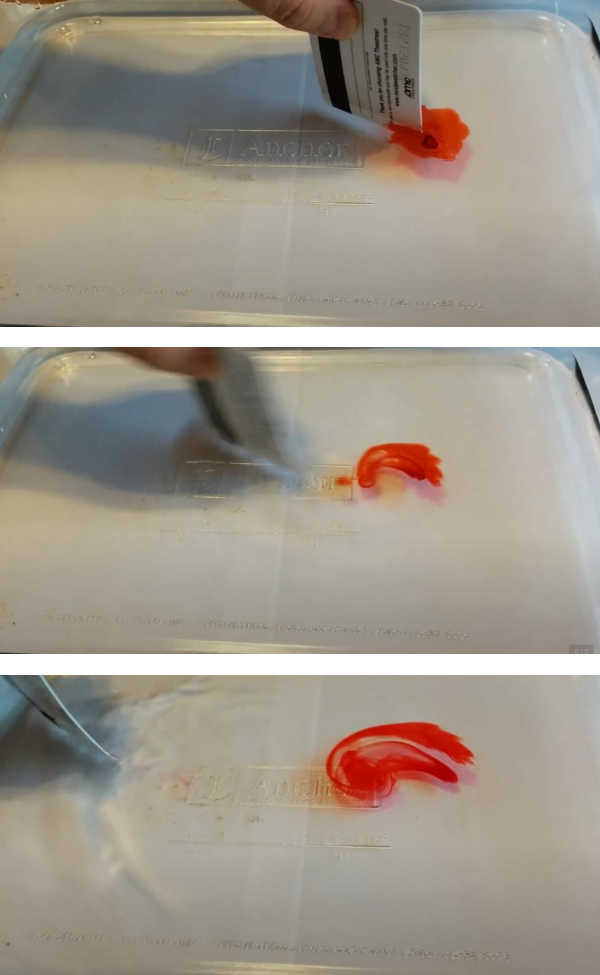
\includegraphics[width=0.8\linewidth]{Figures/Chapter4/fig_starting_vortex}
\caption{Put some water in a shallow container, place a small plastic card in the fluid, and put a small drop of food colouring at the edge of the card.  Drag the card to the left, keeping the angle of attack consistent, and the dye will trace out the starting vortex.}
\label{fig_starting_vortex}
\end{figure}

%
%  SECTION 4.3 - VORTEX MOTION
%

\section{Vortex Motion}

% SECTION 4.3.1 - THE HELMHOLTZ VORTEX THEOREMS

\subsection{The Helmholtz Vortex Theorems}

We've investigated flows involving vorticity throughout the book, and the time has come to properly define a \emph{vortex line} -- not quite the same thing as a line vortex flow -- and a \emph{vortex tube}.  

A vortex line is a curve in the fluid which, at some time $t$, has the same direction as the vorticity,
\[
\vec{\omega} = \grad \times \vec{u}
\]
at each point (see left panel of Figure \ref{fig_vortex_tube}).  Essentially that makes vortex lines similar to stream lines, but for vorticity $\vec{\omega}$ rather than the velocity $\vec{u}$.  A vortex tube is a bundle of vortex lines -- it's formed, again at some time $t$, by all vortex lines passing through a closed curve $C_1$ (see the right panel of Figure \ref{fig_vortex_tube}).  

\begin{figure}
\centering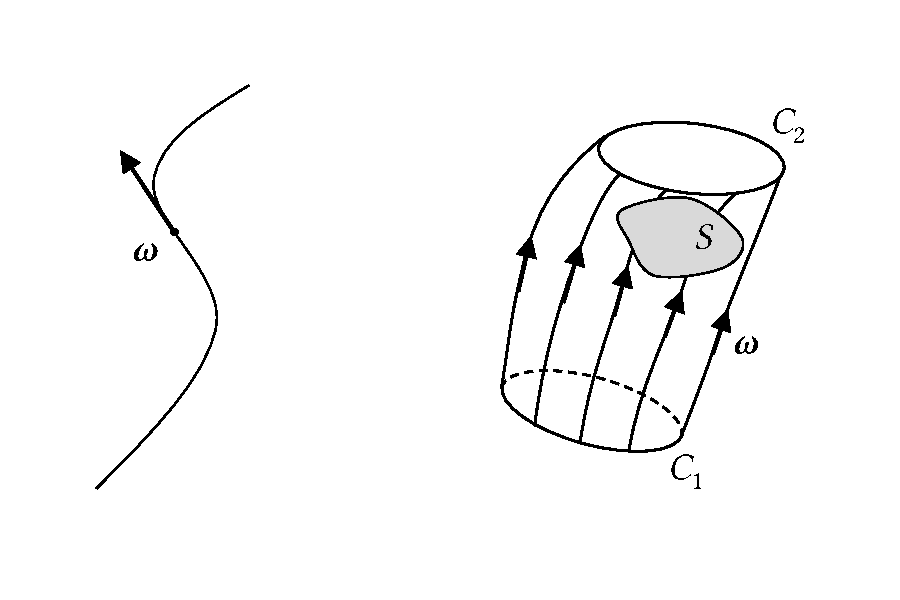
\includegraphics[width=0.8\linewidth]{Figures/Chapter4/fig_vortex_tube}
\caption{Left: The tangent of each point on a vortex line has the same direction as the vorticity $\vec{\omega}$.  Right: A vortex tube is the collection of vortex lines that lie along a closed curve in the fluid.}
\label{fig_vortex_tube}
\end{figure}

For an ideal fluid, Helmholtz formulated a number of theorems\footnote{I've seen textbooks list two, three, or four theorems; I'll state three here, but the essential ideas are all the same.} about the appearance and motion of vortex lines and tubes:

\begin{theorem}[Helmoholtz's Vortex Theorems]
\begin{enumerate}
\item Vortex lines move with the fluid.
\item The strength of a vortex tube is constant.
\item A vortex tube cannot end within the fluid -- it must end on a solid boundary, a free surface, or form a closed loop.
\end{enumerate}
\end{theorem}

Of these, the first is most important to our purpose here, and I'll sketch a brief proof.  Consider the surface $S$ on the vortex tube as shown in Figure \ref{fig_vortex_tube} -- $S$ is on the surface of the vortex tube itself, so that its area vector $\unit{n}$ is perpendicular to the vorticity $\vec{\omega}$ of each vortex line.  If that's the case, then the circulation around the perimeter of $S$ must be zero. We can see this from equation (\ref{eq_circ_curl}), which says the circulation can be calculated from
\[
\Gamma = \int_S \vec{\omega} \cdot d\vec{a}.
\]
Since the area vector is always perpendicular to the vorticity, the dot product is zero and $\Gamma = 0$ around this surface.  Kelvin's circulation theorem ensures that $\Gamma = 0$ always for the surface $S$, so that even as the fluid moves, $S$ remains on the surface of the vortex tube; since $S$ is an arbitrary surface and could be anywhere, the conclusion is that as the fluid moves, the vortex tube remains a vortex tube and moves with the fluid.  Taking the vortex tube to be infinitesimally thin gives us a vortex line, proving Helmholtz's first theorem.

% SECTION 4.3.2 - A VORTEX PAIR

\subsection{A Vortex Pair}

The practical result of this theorem can be seen by considering two vortexes, separated by a distance $2d$ and having opposite circulation but equal strength; this is the same flow we've seen before for a vortex beside a wall (Section \ref{sec_images}), but here we'll actually consider both vortexes in the fluid.  Helmholtz's first theorem says that each vortex will move with the fluid -- in this case, the vortex on the left will have an effect on the one on the right, and vice versa.  To see what effect they have on each other, take a look at Figure \ref{fig_vortex_pair1} and consider first the left vortex.  The fluid velocity due to it is given by
\[
\vec{u} = \frac{\Gamma}{2\pi s} \, \unit{\phi},
\]
which at the position of the right vortex is
\[
\vec{u} = -\frac{\Gamma}{4\pi d} \, \unit{y}.
\]
Evidently, the left vortex causes the right vortex to move \emph{down} along the negative $y$ direction.  Note that the right vortex has no effect on itself -- it can't push on itself any more than a charged particle can create an electric force on itself. 

\begin{figure}
\centering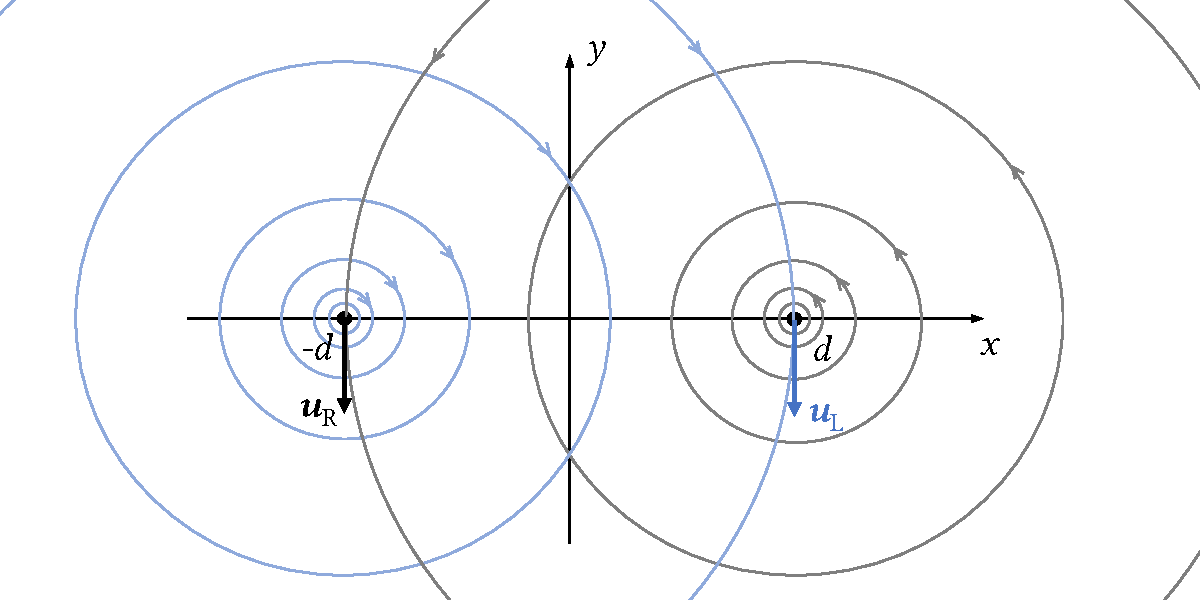
\includegraphics[width=0.8\linewidth]{Figures/Chapter4/fig_vortex_pair1}
\caption{Two vortexes of equal but opposite circulation, a distance $2d$ apart.  The left vortex induces a fluid velocity $\vec{u}_\text{L}$ at the position of the right vortex, and the right vortex induces a velocity $\vec{u}_\text{R}$ at the left.}
\label{fig_vortex_pair1}
\end{figure}

If we look at the effect of the right vortex on the left, we get a similar result:  the right causes the left to move downward with the same speed.  Both vortexes move together, in lockstep, with speed
\begin{equation}
V = \frac{\Gamma}{4\pi d}.
\end{equation}
It's actually quite easy to create a vortex pair like this; dragging a small plate through water will do it, with a vortex formed at each edge of the plate.  Once the plate is removed, the vortexes will continue to move due to each other's influence.  Figure \ref{fig_vortex_pair_pool} shows a vortex pair moving across a small pool.

\begin{figure}
\centering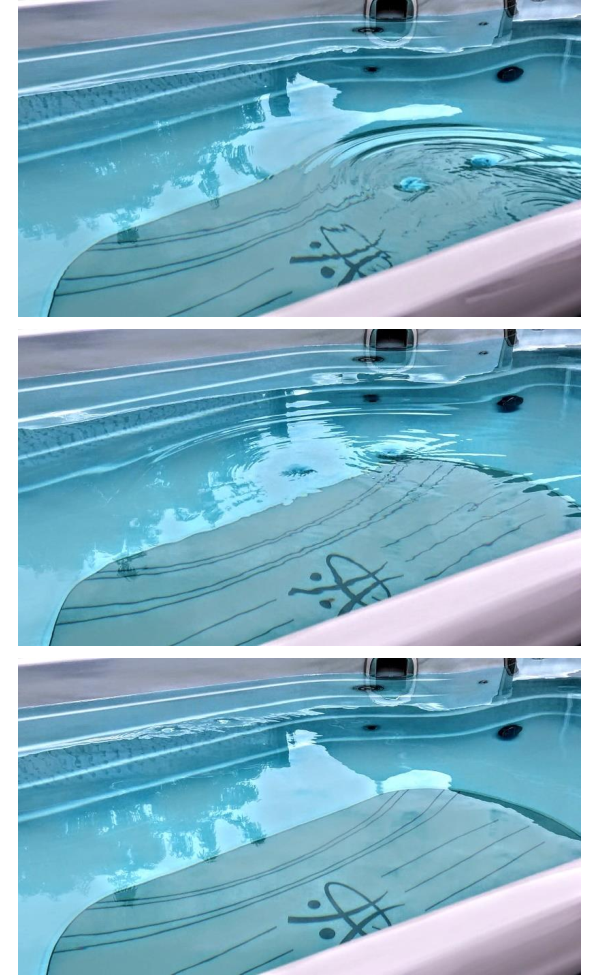
\includegraphics[width=0.9\linewidth]{Figures/Chapter4/fig_vortex_pair_pool}
\caption{It's possible to create a vortex pair by dragging a small plate through a pool of water.  The starting vortexes that form are equal in strength and opposite in direction, and they travel across the pool at constant speed and without losing strength.}
\label{fig_vortex_pair_pool}
\end{figure}

If we want to model the vortex pair, we can shift to a reference frame in which they are at rest so that the overall flow is steady.  That means we'll need to include, in addition to the two vortexes, a uniform flow with speed $V$ moving upward.  The complex potential of uniform flow is
\[
w_\text{uni}(z) = Uze^{-i\alpha},
\]
and to have the flow move upward along $+\unit{y}$, we'll set $\alpha = \pi/2$, so that $e^{-i\pi/2} = -i$.  With $U = V = \Gamma/4\pi d$ we have
\[
w_\text{uni}(z) = -\frac{i\Gamma z}{4\pi d}.
\]
The full complex potential, including the two opposite but equal vortexes, would be
\begin{equation}
w(z) = -\frac{i\Gamma z}{4\pi d} - \frac{i\Gamma}{2\pi} \ln (z-d) + \frac{i\Gamma}{2\pi} \ln (z+d),
\end{equation}
and streamlines for this flow are shown in Figure \ref{fig_vortex_pair3}.

\begin{figure}
\centering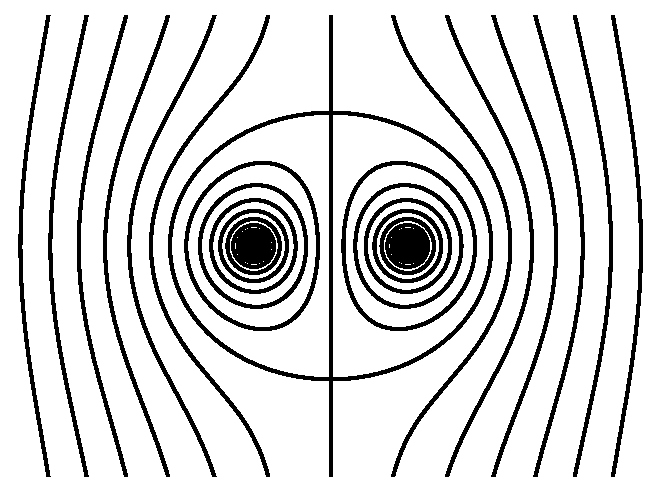
\includegraphics[width=0.7\linewidth]{Figures/Chapter4/fig_vortex_pair3}
\caption{Streamlines for the flow in a reference frame in which the vortex pair is at rest.}
\label{fig_vortex_pair3}
\end{figure}

Are the vortexes actually at rest in this reference frame?  We can check easily enough by calculating their speed.  Let's start with the derivative of the complex potential,
\begin{equation}
\label{eq_vortex_pair}
\frac{dw}{dz} = u - iv = -\frac{i\Gamma}{4 \pi d} - \frac{i\Gamma}{2\pi} \frac{1}{z-d} +  \frac{i\Gamma}{2\pi} \frac{1}{z+d}.
\end{equation}
To find the speed of the vortex on the right, we evaluate this derivative at its location, $z = d$:
\[
u_R - iv_R = \left. \frac{dw}{dz} \right|_{z=d}.
\]
But be careful here: the right vortex won't be affected by itself, so we'll ignore that particular term --the second -- in equation (\ref{eq_vortex_pair}).  The speed of the right vortex becomes
\[
u_R - iv_R = -\frac{i\Gamma}{4\pi d} + \frac{i\Gamma}{2\pi} \left( \frac{1}{2d} \right) = 0.
\]
So, as expected, $u_R = 0$ and $v_R = 0$ -- the vortex on the right is at rest in this reference frame.  Similarly for the vortex on the left.


% SECTION 4.3.3 - VORTEX SHEDDING

\subsection{Vortex Shedding}

We've been discussing ideal fluids exclusively for the last two chapters, and will continue with them for the next one as well.  But I want to return for a moment to the major difference between viscous and inviscid flow at high Reynolds number: the presence of a boundary layer.  In an ideal fluid, flow around a circular cylinder looks like our solution (Figures \ref{fig_uniform_circle} and \ref{fig_cylinder_circ}) regardless of how fast the fluid is flowing.  In reality, for high speed flow (or equivalently high Reynolds number flow), the viscous boundary layer plays an important role in the behaviour of the fluid downstream.  

\begin{figure}
\centering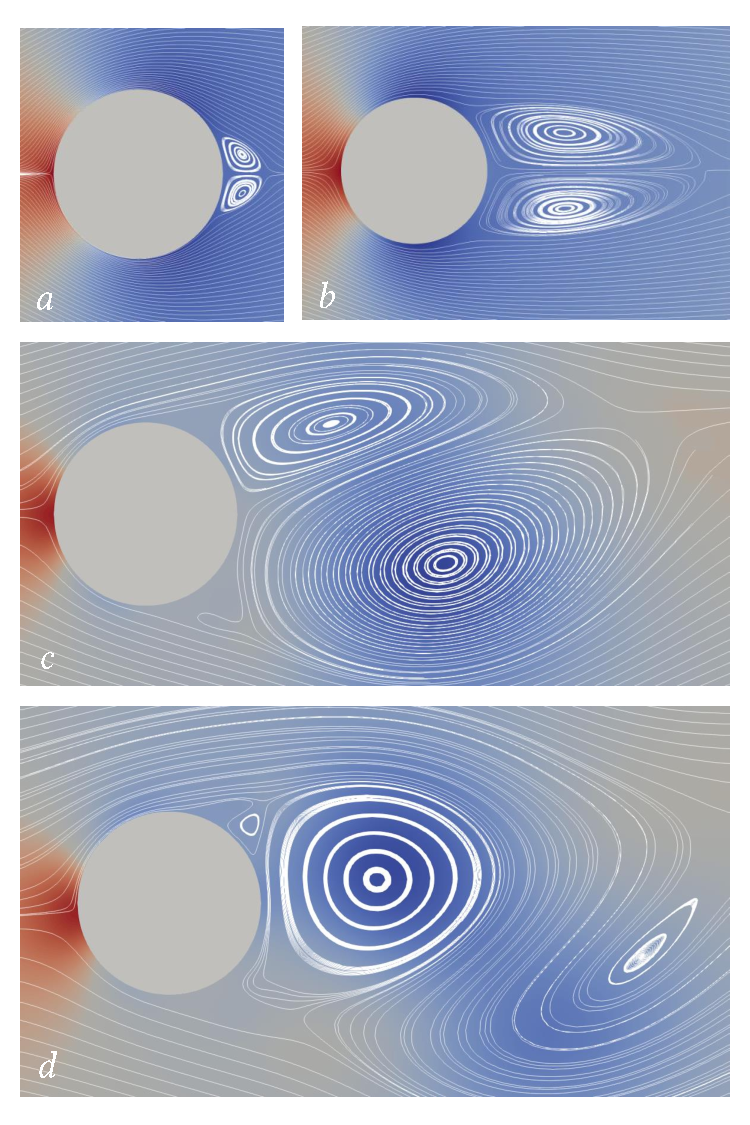
\includegraphics[width=0.9\linewidth]{Figures/Chapter4/fig_vortex_shedding}
\caption{Computational fluid dynamics simulation past a circular cylinder.  The popular open source code SU2 was used.  (a) Reynolds number $R = 10$.  A vortex pair is formed on the trailing side shortly after the flow is started.  (b) $R = 30$.  The region in which the fluid reverses is larger.  (c) and (d) $R = 10,000$.  The flow becomes unsteady and asymmetric (c), and eventually (d) the vortexes begin to detach and are shed downstream.}
\label{fig_vortex_shedding}
\end{figure}

To illustrate this, Figure \ref{fig_vortex_shedding} shows a computational fluid dynamics simulation of viscous flow past a circular cylinder.  At low Reynolds number (between five to 40 or so), the boundary layer at the trailing edge of the surface grows; this boundary layer is high in vorticity and eventually two small vortexes appear.  These vortexes are equal in strength and opposite in direction -- the flow \emph{reverses} near the trailing stagnation point.  Figure \ref{fig_vortex_shedding}$a$ shows the vortexes for $R = 10$; at slightly higher Reynolds number ($R = 30$) these vortexes are larger as in Figure \ref{fig_vortex_shedding}$b$.  However, at Reynolds number greater than around 40, something interesting happens:  the vortexes become \emph{unstable} and one grows in size over the other (Figure \ref{fig_vortex_shedding}$c$).  The larger vortex then detaches from the cylinder and travels downstream (Figure \ref{fig_vortex_shedding}$d$), forming a wake.  This process is called \emph{vortex shedding}, and the wake has a highly structured form, something we'll consider in depth in a moment.  

Before we consider the wake, however, I'd like to try modelling the initial phase of vortex shedding -- the steady vortexes that are attached to the trailing edge of the cylinder.  We can approximate these attached vortexes as ideal line vortexes, but it turns out that adding them to a circular cylinder is a little difficult.  Instead, we can simplify the situation a by using a flat boundary at $x = 0$, as shown in Figure \ref{fig_attached_vortex1}.  Now, that's definitely not a curved circular surface, but as long as we imagine the circle is large and the vortexes close to it, it doesn't do too bad a job.

\begin{figure}
\centering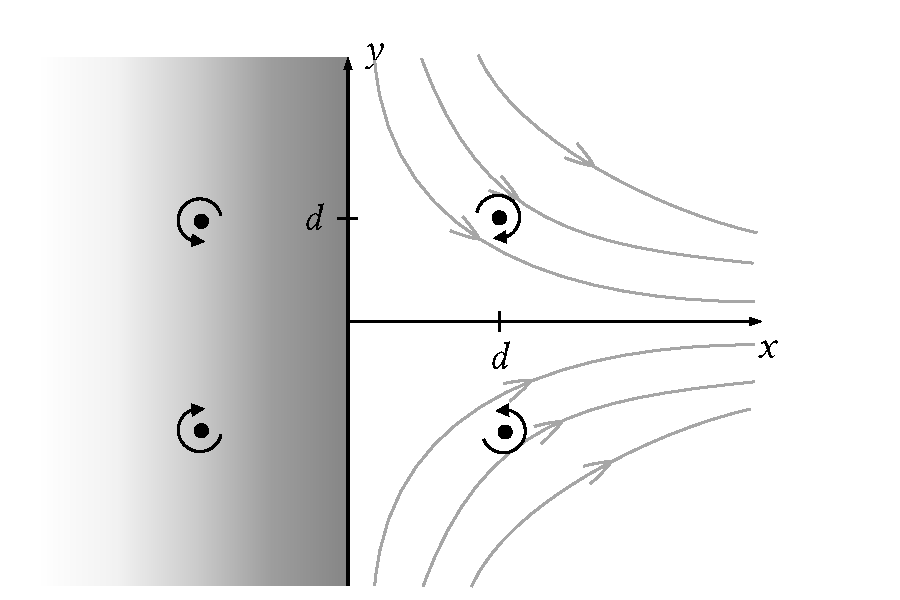
\includegraphics[width=0.75\linewidth]{Figures/Chapter4/fig_attached_vortex1}
\caption{Modelling the attached vortexes requires mirror images for each.  Note the circulation directions and positions of each vortex.}
\label{fig_attached_vortex1}
\end{figure}

We can model the flow around the ``circle'' with the stagnation point flow, 
\[
w(z) = \frac{1}{2} \alpha z^2,
\]
as shown in the light grey lines in Figure \ref{fig_attached_vortex1}.  The vortexes will be added to this flow, but we have to be careful.  There's a boundary at $x=0$ and we must ensure the flow meets the boundary conditions there -- that is, it has to slip along that wall.  But we already know how to handle this -- with method of images.  So in addition to the two vortexes we want in our flow, we also need two mirror vortexes on the other side of the wall with opposite circulation; that will give us the correct boundary, as you can check for yourself.  So, we need four vortexes, all the same strength, but with two having counterclockwise circulation (positive $\Gamma$) and two having clockwise (negative $\Gamma$).  Setting the position $z_0$ of the top right vortex fixes all the others in place.  If
\[
z_0 = d + id,
\]
then the lower right vortex is at $d - id = z_0^*$, the upper left is at $-d + id = -z_0^*$, and the lower left vortex is at $-d -id = -z_0$.  The full complex potential, including the background stagnation point flow, will be
\begin{equation}
\label{eq_w_vortex_shedding}
w(z) = \frac{1}{2} \alpha z^2 + \frac{i\Gamma}{2\pi} \ln (z - z_0) -  \frac{i\Gamma}{2\pi} \ln (z - z_0^*) -  \frac{i\Gamma}{2\pi} \ln (z + z_0^*) +  \frac{i\Gamma}{2\pi} \ln (z + z_0).
\end{equation}

Only for one particular choice of $d$, however, will the vortexes be at rest -- and so ``attached'' to the cylinder.  Problem \ref{prob_attached_vortexes} asks you to find this; the answer is
\begin{equation}
d = \sqrt{\frac{\Gamma}{8 \pi \alpha}}.
\end{equation}
Once we have the correct complex potential, we can find the streamlines from $\phi = \operatorname{Im}(w)$ as usual, and, if we want, the pressure from Bernoulli's theorem.  Figure \ref{fig_attached_vortex2} shows the vortexes and pressure; it's up to you to compare with Figure \ref{fig_vortex_shedding} and see if our model does a reasonable job at reproducing it.  Note, however, that although the vortexes are \emph{steady} when placed at $d \pm id$, they're also \emph{unstable} and would detach with any kind of perturbation.

\begin{figure}
\centering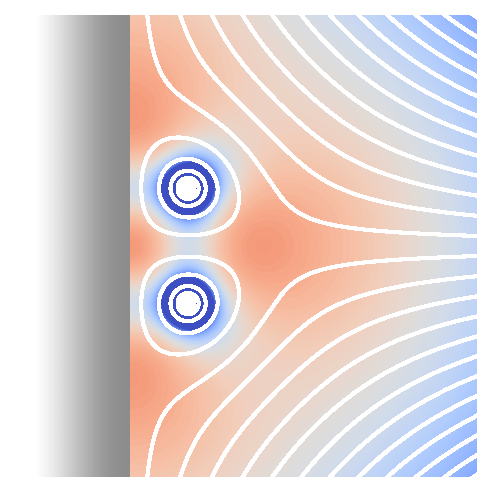
\includegraphics[width=0.5\linewidth]{Figures/Chapter4/fig_attached_vortex2}
\caption{Streamlines and pressure field for the attached vortexes.}
\label{fig_attached_vortex2}
\end{figure}


% SECTION 4.3.4 - VON KARMAN VORTEX STREET

\subsection{The von K\'arm\'an Vortex Street}

Under the right conditions, the wake created by vortex shedding from a cylinder or other object can be highly structured and periodic -- the vortexes form a \emph{von K\'arm\'an vortex street,}  in which vortexes travel downstream from the object in two separate lines.  This is frequently seen in nature when wind blows past an island mountain in the ocean and surrounding clouds form the vortex street; examples are shown in Figure \ref{fig_vortex_street_clouds}.  It's also readily seen in fluid simulations such as the one in Figure \ref{fig_vortex_shedding}, and, since it is at least approximately steady state, it's amenable to a simple model.

\begin{figure}
\centering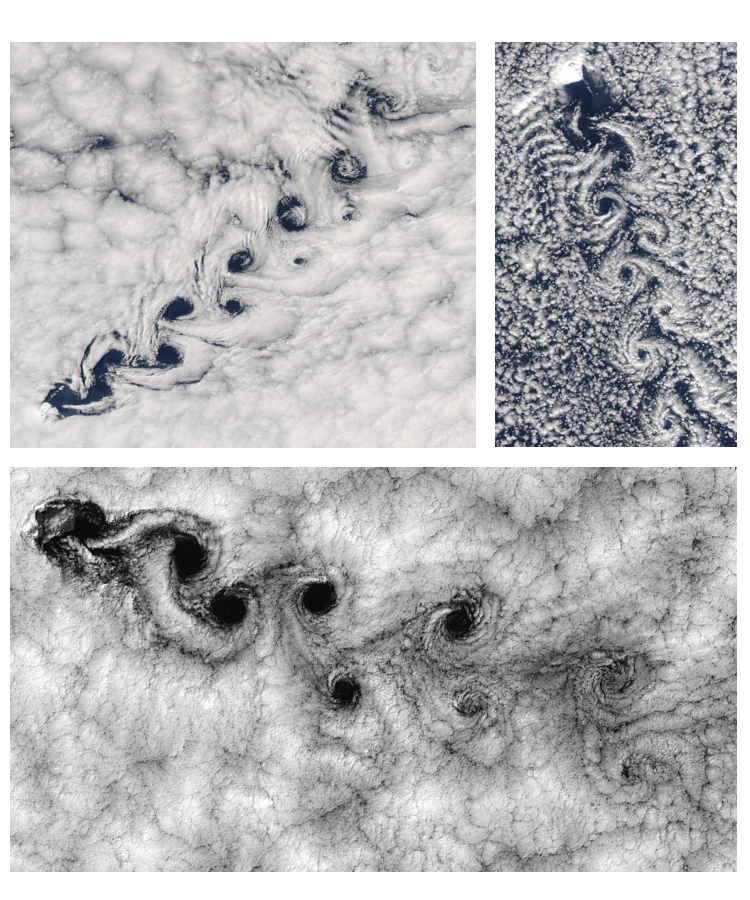
\includegraphics[width=0.9\linewidth]{Figures/Chapter4/fig_vortex_street_clouds}
\caption{Examples of vortex streets forming in clouds as the air moves past islands in the ocean.  All photos from NASA.}
\label{fig_vortex_street_clouds}
\end{figure}

As we did above, we'll model each vortex in the street as a line vortex, but since we're approximating this as a steady state, we'll need an infinite number of them in two rows.  Imagine that an object exists far to the left, and uniform flow to the right past this object creates a vortex street.  We'll stagger the vortexes as shown in Figure \ref{fig_vortex_street1}.  Note the orientation of each vortex -- along the top row, they have clockwise (negative $\Gamma$) circulation, while each vortex in the bottom row circulates in a counterclockwise (positive $\Gamma$) fashion.  Each vortex is separated by their neighbours in their line by a distance $a$, the the two lines are separated by a distance $b$.


\begin{figure}
\centering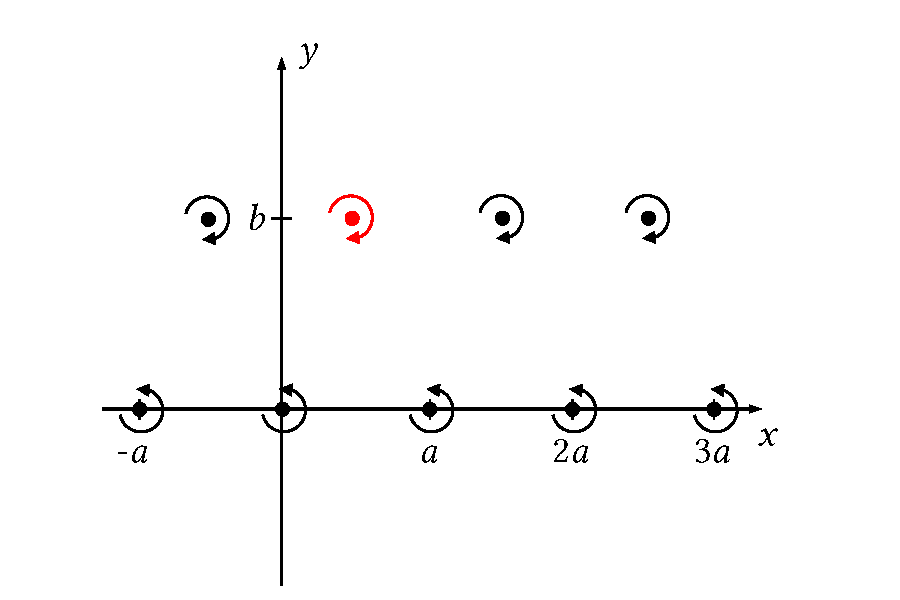
\includegraphics[width=0.7\linewidth]{Figures/Chapter4/fig_vortex_street1}
\caption{Model of a vortex street:  two infinite lines of vortexes, with each line having opposite rotation.}
\label{fig_vortex_street1}
\end{figure}


Our objective will be to find the complex potential that describes the flow, but first we need to think about how this vortex street \emph{moves}.  Consider just one vortex -- the red one in Figure \ref{fig_vortex_street1}, which is located in the complex plane at 
\[
z = \frac{1}{2} a + ib.
\]
Remember, each of the vortexes in the street will move due to the influence of all the rest.  But for this vortex, the others  in the top row will have no effect -- because they're evenly spaced, they cancel in pairs, and the net result is that the fluid is at rest at the location of the red vortex.  The bottom row, however, does have an effect.  With a little bit of thought, you should be able to see that the fluid velocity at the position of the red vortex due to the bottom row is to the \emph{left}.

That the flow is to the left might sound strange at first -- we set up this problem so that the object creating the vortex street is far to the left and the flow is moving to the right.  But right now we're in the reference frame of the uniform flow itself -- we're moving to the right with it, and the vortexes in the street evidently move to the left in this frame.  That means that in the reference frame where the object is at rest, the vortexes will move to the \emph{right}, but more slowly than the uniform flow past the object.  We'll stick with the uniform flow reference frame for now, but can always add in a uniform flow later if we want to.

What exactly is the speed the vortexes move with?  To answer, we'll have to write down the complex potential for the bottom row -- I'll ignore the top row for now since it has no effect on the red vortex we're examining.  In principle the complex potential is simple to write down, although there are an infinite number of vortexes:
\[
w(z) = \cdots - \frac{i\Gamma}{2\pi} \ln (z + a) - \frac{i\Gamma}{2\pi} \ln (z) - \frac{i\Gamma}{2\pi} \ln (z - a) - \cdots
\]
Now, the $n$th term is
\[
w_n(z) = -\frac{i\Gamma}{2\pi} \ln (z - na),
\]
and $n$ will run from $-\infty$ to $\infty$.  But we can write this instead as
\[
w_n(z) = -\frac{i\Gamma}{2\pi} \ln \left(1 - \frac{z}{na} \right);
\]
it differs from the above only by a constant, which isn't important for the complex potential.  Then the full complex potential due to the bottom row is
\begin{equation}
w(z) = -\frac{i\Gamma}{2\pi} \sum_{n=-\infty}^{-1} \ln \left(1 - \frac{z}{na} \right) - \frac{i\Gamma}{2\pi} \ln z -\frac{i\Gamma}{2\pi} \sum_{n=1}^{\infty} \ln \left(1 - \frac{z}{na} \right).
\end{equation}
The first term handles all the vortexes to the left of the origin, the middle term the vortex at the origin itself, and the right term the vortexes to the right.  

This is correct, but we can simplify it quite a bit by doing some rearranging.  I'll write out some of the terms so we can see the pattern we're looking for better:
\begin{multline*}
w(z) = -\frac{i\Gamma}{2\pi} \biggl[ \ln z + \cdots + \ln \left(1 - \frac{z}{(-2a)} \right) +  \ln \left(1 - \frac{z}{(-a)} \right) + \\ \ln \left(1 - \frac{z}{a} \right) +  \ln \left(1 - \frac{z}{2a} \right) + \cdots \biggr]
\end{multline*}
We can use log rules to turn those additions of logs to multiplications within, getting
\[
w(z) = -\frac{i\Gamma}{2\pi} \ln \biggl[ (z) \cdots \left(1 - \frac{z}{(-2a)} \right) \left(1 - \frac{z}{(-a)} \right) \left(1 - \frac{z}{(a)} \right) \left(1 - \frac{z}{(2a)} \right) \cdots \biggr]
\]
At this point we can do some of the multiplication.  Consider the inner two terms - if we multiply them together we get a difference of squares,
\[
\left(1 - \frac{z}{(-a)} \right) \left(1 - \frac{z}{(a)} \right) = \left( 1 - \frac{z^2}{a^2} \right),
\]
and similarly with the outer two terms.  In fact, along the entire infinite number of terms, we can combine them in pairs so that we get
\[
w(z) = -\frac{i\Gamma}{2\pi} \ln \biggl[ z \prod_{n=1}^\infty \left( 1- \frac{z^2}{n^2 a^2} \right) \biggr].
\]
It turns out the thing in the square brackets is actually an infinite product expansion of the sine function, and we finally have 
\begin{equation}
\label{eq_vortex_street}
w(z) = -\frac{i\Gamma}{2\pi}\ln \biggl[ \sin \left( \frac{\pi z}{a} \right) \biggr].
\end{equation}

\begin{figure}
\centering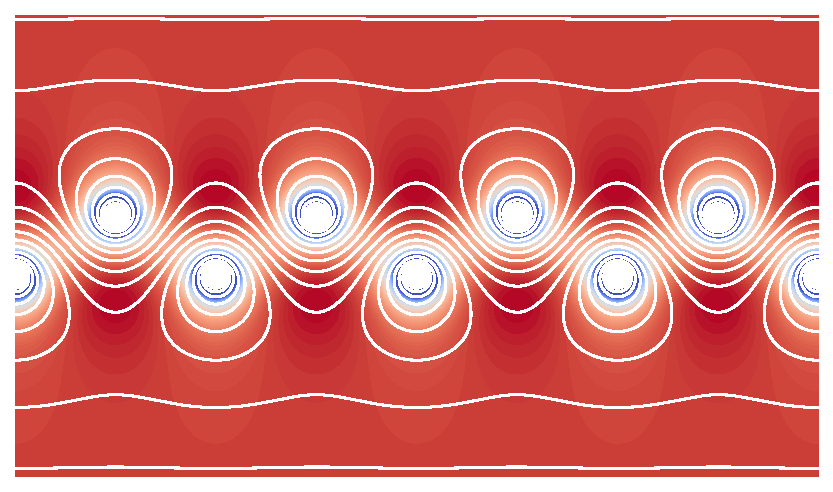
\includegraphics[width=0.95\linewidth]{Figures/Chapter4/fig_vortex_street2}
\caption{Streamlines and pressure of the simple model for the vortex street.  Here $a = 1$ and $b = 0.2$ and the uniform flow velocity is $U = u_0$ so that the vortexes are at rest in this frame. }
\label{fig_vortex_street2}
\end{figure}

Now we can easily get the speed of the red vortex in Figure \ref{fig_vortex_street1}.  Taking the derivative gives
\[
u - iv = \frac{dw}{dz} = -\frac{i\Gamma}{2\pi} \cot \left( \frac{\pi z}{a} \right).
\]
This is the velocity of the fluid everywhere due to the bottom row only.  If we evaluate this at the location of the red vortex, $z = \tfrac{1}{2} a + ib$, we find
\[
u_0 - iv_0 = \left. \frac{dw}{dz} \right|_{z = \tfrac{1}{2} a + ib} = -\frac{\Gamma}{2a} \tanh \left( \frac{\pi b }{a} \right).
\]
That means the velocity components of the vortex are
\begin{equation}
\label{eq_vortex_street_speed}
u_0 = -\frac{\Gamma}{2a} \tanh \left( \frac{\pi b }{a} \right) \quad \text{and} \quad v_0 = 0.
\end{equation}
As expected, it moves to the left ($u_0$ is negative) and has no motion along the $y$ direction (see Problem \ref{prob_vortex_street}).

Now that we've analyzed the bottom row, we can easily repeat for the top to find the total complex potential.  The full complex potential everywhere is
\begin{equation}
w(z) = -\frac{i\Gamma}{2\pi}\ln \biggl[ \sin \left( \frac{\pi z}{a} \right) \biggr] + \frac{i\Gamma}{2\pi}\ln \biggl[ \sin \left( \frac{\pi (z - a/2 - ib)}{a} \right) \biggr] + Uz,
\end{equation}
where the last term allows for a uniform flow if we want to move to a reference frame in which it has a non-zero velocity.  Figure \ref{fig_vortex_street2} shows the streamlines and pressure for this complex potential, and I set $U = -u_0$, the speed at which the vortexes travel, so that they are at rest in the figure.  Again, it's up to you to decide how good the model is; compare with the cloud photographs or simulation images.




\section*{Problems}
\addcontentsline{toc}{section}{Problems}
\markright{Problems}%

\begin{problem}[Complex numbers]

(a) Show that $|z|^2$ is real using polar coordinates.

(b) Show that $1/i = -i$.

(c) Show that
\[
\sqrt{i} = \frac{1}{\sqrt{2}} + \frac{i}{\sqrt{2}}.
\]
\end{problem}


\begin{problem}[A line source]
\label{prob_line_source_w}
Starting from the velocity potential $\varphi(s, \phi)$ and stream function $\psi(s, \phi)$ , derive the complex potential for a line source of strength $Q$.
\end{problem}


\begin{problem}[Power law complex potentials]
Consider a general complex potential of the form $w(z) = Az^n$.  For $n = 2/3, 3/2, 2,$ and $n = 3$, plot the streamlines and physically interpret the flow.  Is there a relationship between the exponent $n$ and how the flow behaves?
\end{problem}

\begin{problem}[The doublet flow]
Of special interest is the power law flow with $n = -1$: $w(z) = A/z$.  For this flow, find the velocity potential and stream function as well as the velocity (use polar coordinates).  Plot the streamlines.
\end{problem}

\begin{problem}[Combination of flows]
Plot the streamlines for a flow that consists of a stagnation point of strength $\alpha = 1$ and a line vortex of strength $\Gamma = 10$ and positioned at $z = 1$.
\end{problem}

\begin{problem}[Boundary conditions from the mirror image]
\label{prob_mirror_bc}
Starting from equation (\ref{eq_mirror_vortex}), find the velocity of the fluid $[u, v]$ and show that the flow slips along the wall (in other words, shown that $u(0, y) = 0$).  Warning:  this will take a fair bit of algebra.
\end{problem}

\begin{problem}[A vortex in a corner]
Consider a vortex located at $z = a + ib$, where $a$ and $b$ are both positive, and there are boundaries as shown in Figure \ref{fig_vortex_corner}.  

(a) What is the complex potential for the fluid in the region $x \ge 0, y \ge 0$?

(b) Plot the streamlines for the region $x \ge 0, y \ge 0$.

(c) Show explicitly that the fluid velocity is zero at the corner.

(d) This vortex will \emph{move} due to the rest of the flow.  Show that the path the vortex takes is given by
\[
\frac{1}{x} + \frac{1}{y} = \text{constant}.
\]
\end{problem}

\begin{figure}
\centering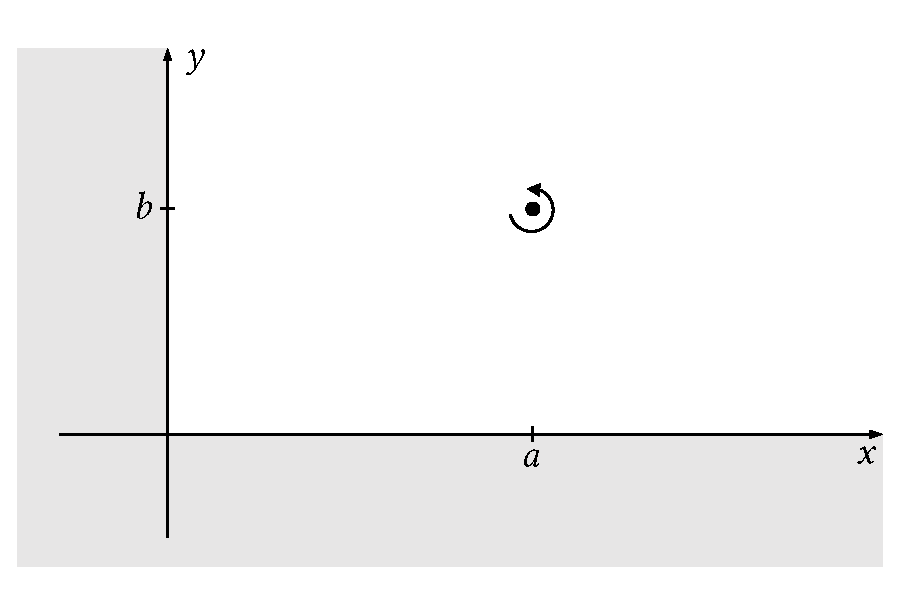
\includegraphics[width=0.75\linewidth]{Figures/Chapter4/fig_vortex_corner}
\caption{A line vortex in a corner.}
\label{fig_vortex_corner}
\end{figure}

\begin{problem}[A line source by a wall]
Consider a line source $Q$ a distance $b$ from a boundary along $x = 0$ (so the fluid exists only in $x>0$).  Use the method of images to determine the complex potential, making sure to show explicitly that the boundary condition is satisfied (a drawing will do).  Then find the velocity $u$ of the flow and plot the streamlines.
\end{problem}

\begin{problem}[A line source by two walls]
Suppose there are two boundaries, one at $y = +b$ and one at $y = -b$, with fluid in between.  A line source $Q$ sits right in the middle at $y = 0$.  Show that the complex potential is
\[
w(z) = \frac{Q}{2\pi} \ln \left[ \sinh \left( \pi z / 2b \right) \right].
\]
\end{problem}

\begin{problem}[Using the circle theorem]
Consider the complex potential
\[
w(z) = \frac{A}{2} (z^2 - 2cz)
\]
where $A$ and $c$ are constants.  

(a) Find the velocity potential and the stream function and plot the streamlines.

(b) Add a circular cylinder to the flow using the Milne-Thomson circle theorem and find the new complex potential.  Show that the stream function is given by
\[
\psi(x, y) = Ay \left[ x \left( 1 + \frac{a^2}{x^2 + y^2} \right) - c\right] \left(1 - \frac{a^2}{x^2 + y^2} \right)
\]
and plot the new streamlines.
\end{problem}

\begin{problem}[Flow around a circular cylinder]
\label{prob_circlular_cylinder}
Equation (\ref{eq_uniform_circle}) gives the complex potential for flow around a circular cylinder, including an angle and circulation, but for this problem set $\alpha = 0$.  

(a) By taking the derivative of $w(z)$, show that the velocity is given by
\[
u_s(s, \phi) = U \left( 1 - \frac{a^2}{s^2} \right) \cos \phi \quad \text{and} \quad u_\phi(s, \phi) = -U \left( 1 + \frac{a^2}{s^2} \right) \sin \phi + \frac{\Gamma}{2\pi s}.
\]

(b) Show that there are two stagnation points on the cylinder (at $s = a$) if the circulation is $\Gamma < 4\pi U a$, only one point if $\Gamma = 4\pi U a$, and none if $\Gamma > 4\pi U a$. 

(c) Where is the stagnation point in the fluid if $\Gamma = 8 \pi U a$?  (Hint: it's not on the boundary $s=a$.)
\end{problem}

\begin{problem}[Force on a circular cylinder]
\label{prob_force2}
Problem \ref{prob_force1} asked you to calculate the force on a cylinder from an ideal fluid.  Repeat that calculation, but this time include \emph{circulation} $\Gamma$ (you can set $\alpha = 0$, though), and show that
\[
F_x = 0 \quad \text{and} \quad F_y = -\rho U \Gamma.
\]
\end{problem}

\begin{problem}[Flow around an ellipse and a flat plate]
\label{prob_flat_plate}

(a) Starting from the complex potential for flow past a circular cylinder (equation \ref{eq_uniform_circle}), use the inverse Joukowski transform to derive the flow past an elliptical cylinder (equation \ref{eq_ellipse_w}).

(b) With $c = a$ in the Joulowski transform, the ellipse becomes a flat plate.  Using equation (\ref{eq_dwdz}), show that the singularity in the flow at $z = +a$ disappears if the circulation is $\Gamma = -4\pi U a \sin \alpha$, and show that the flow at that point is
\[
\U = U \cos \alpha \quad \text{and} \quad \V = 0.
\]
\end{problem}

\begin{problem}[Attached Vortexes]
\label{prob_attached_vortexes}
Equation \ref{eq_w_vortex_shedding} gives the complex potential for a pair of attached vortexes.  By taking the derivative of this expression and evaluating it at the location of each vortex, show that the vortexes are at rest if
\[
d = \sqrt{\frac{\Gamma}{8\pi \alpha}}.
\]
\end{problem}

 
\begin{problem}[The vortex sptreet]
\label{prob_vortex_street}
For the vortex street, the complex potential for the bottom row is given by equation (\ref{eq_vortex_street}).  From this, show that the velocity of the red vortex in Figure \ref{fig_vortex_street1} is given by equation (\ref{eq_vortex_street_speed}).
\end{problem}

